\documentclass[a4paper]{book}
\usepackage{a4wide}
\usepackage{makeidx}
\usepackage{graphicx}
\usepackage{multicol}
\usepackage{float}
\usepackage{listings}
\usepackage{color}
\usepackage{textcomp}
\usepackage{alltt}
\usepackage{times}
\usepackage{ifpdf}
\ifpdf
\usepackage[pdftex,
            pagebackref=true,
            colorlinks=true,
            linkcolor=blue,
            unicode
           ]{hyperref}
\else
\usepackage[ps2pdf,
            pagebackref=true,
            colorlinks=true,
            linkcolor=blue,
            unicode
           ]{hyperref}
\usepackage{pspicture}
\fi
\usepackage[utf8]{inputenc}
\usepackage{doxygen}
\lstset{language=C++,inputencoding=utf8,basicstyle=\footnotesize,breaklines=true,breakatwhitespace=true,tabsize=8,numbers=left }
\makeindex
\setcounter{tocdepth}{3}
\renewcommand{\footrulewidth}{0.4pt}
\begin{document}
\hypersetup{pageanchor=false}
\begin{titlepage}
\vspace*{7cm}
\begin{center}
{\Large registration }\\
\vspace*{1cm}
{\large Generated by Doxygen 1.7.1}\\
\vspace*{0.5cm}
{\small Fri Dec 16 2011 08:57:16}\\
\end{center}
\end{titlepage}
\clearemptydoublepage
\pagenumbering{roman}
\tableofcontents
\clearemptydoublepage
\pagenumbering{arabic}
\hypersetup{pageanchor=true}
\chapter{Class Index}
\section{Class Hierarchy}
This inheritance list is sorted roughly, but not completely, alphabetically:\begin{DoxyCompactList}
\item \contentsline{section}{Capture}{\pageref{classCapture}}{}
\item \contentsline{section}{FeatureContainerInterface}{\pageref{classFeatureContainerInterface}}{}
\begin{DoxyCompactList}
\item \contentsline{section}{FeatureContainer$<$ FeatureType $>$}{\pageref{classFeatureContainer}}{}
\item \contentsline{section}{FeatureContainerInterface\_\-Euclidean$<$ Point $>$}{\pageref{classFeatureContainerInterface__Euclidean}}{}
\begin{DoxyCompactList}
\item \contentsline{section}{Feature\_\-Edges$<$ Point $>$}{\pageref{classFeature__Edges}}{}
\item \contentsline{section}{Feature\_\-FPFH$<$ Point $>$}{\pageref{classFeature__FPFH}}{}
\item \contentsline{section}{Feature\_\-MomentInvariants$<$ Point $>$}{\pageref{classFeature__MomentInvariants}}{}
\item \contentsline{section}{Feature\_\-NARF$<$ Point $>$}{\pageref{classFeature__NARF}}{}
\end{DoxyCompactList}
\end{DoxyCompactList}
\item \contentsline{section}{FilterNode}{\pageref{classFilterNode}}{}
\item \contentsline{section}{GeneralRegistration$<$ Point $>$}{\pageref{classGeneralRegistration}}{}
\begin{DoxyCompactList}
\item \contentsline{section}{Registration\_\-Corrospondence$<$ Point $>$}{\pageref{classRegistration__Corrospondence}}{}
\item \contentsline{section}{Registration\_\-FastSLAM$<$ Point $>$}{\pageref{classRegistration__FastSLAM}}{}
\item \contentsline{section}{Registration\_\-ICP$<$ Point $>$}{\pageref{classRegistration__ICP}}{}
\begin{DoxyCompactList}
\item \contentsline{section}{Registration\_\-ICP\_\-Features$<$ Point $>$}{\pageref{classRegistration__ICP__Features}}{}
\begin{DoxyCompactList}
\item \contentsline{section}{Registration\_\-ICP\_\-Edges$<$ Point $>$}{\pageref{classRegistration__ICP__Edges}}{}
\item \contentsline{section}{Registration\_\-ICP\_\-Features\_\-Extra$<$ Point, FeatureType $>$}{\pageref{classRegistration__ICP__Features__Extra}}{}
\item \contentsline{section}{Registration\_\-ICP\_\-FPFH$<$ Point $>$}{\pageref{classRegistration__ICP__FPFH}}{}
\item \contentsline{section}{Registration\_\-ICP\_\-Moments$<$ Point $>$}{\pageref{classRegistration__ICP__Moments}}{}
\item \contentsline{section}{Registration\_\-ICP\_\-NARF$<$ Point $>$}{\pageref{classRegistration__ICP__NARF}}{}
\end{DoxyCompactList}
\item \contentsline{section}{Registration\_\-ICP\_\-Features$<$ Point $>$}{\pageref{classRegistration__ICP__Features}}{}
\end{DoxyCompactList}
\item \contentsline{section}{Registration\_\-Infobased$<$ Point $>$}{\pageref{classRegistration__Infobased}}{}
\item \contentsline{section}{Registration\_\-RGBDSLAM$<$ Point $>$}{\pageref{classRegistration__RGBDSLAM}}{}
\end{DoxyCompactList}
\item \contentsline{section}{GeneralSLAM$<$ Point $>$}{\pageref{classGeneralSLAM_3_01Point_01_4}}{}
\item \contentsline{section}{IterativeClosestPoint}{\pageref{classpcl_1_1IterativeClosestPoint}}{}
\begin{DoxyCompactList}
\item \contentsline{section}{ModifiedICP\_\-T$<$ pcl::IterativeClosestPoint$<$ PointT, PointT $>$, PointT $>$}{\pageref{classModifiedICP__T}}{}
\begin{DoxyCompactList}
\item \contentsline{section}{ModifiedICP$<$ PointT $>$}{\pageref{classModifiedICP}}{}
\end{DoxyCompactList}
\end{DoxyCompactList}
\item \contentsline{section}{preprocessing::KinectErrorGenerator$<$ PointT $>$}{\pageref{classpreprocessing_1_1KinectErrorGenerator}}{}
\item \contentsline{section}{MemoryOperator}{\pageref{classMemoryOperator}}{}
\item \contentsline{section}{measurement\_\-tools::MemoryUsage}{\pageref{classmeasurement__tools_1_1MemoryUsage}}{}
\item \contentsline{section}{ModifiedICP\_\-G}{\pageref{classModifiedICP__G}}{}
\begin{DoxyCompactList}
\item \contentsline{section}{ModifiedICP\_\-T$<$ ParentClass, PointT $>$}{\pageref{classModifiedICP__T}}{}
\item \contentsline{section}{ModifiedICP\_\-T$<$ pcl::IterativeClosestPoint$<$ PointT, PointT $>$, PointT $>$}{\pageref{classModifiedICP__T}}{}
\end{DoxyCompactList}
\item \contentsline{section}{NarfKPoint}{\pageref{structNarfKPoint}}{}
\item \contentsline{section}{ParameterBag}{\pageref{classParameterBag}}{}
\begin{DoxyCompactList}
\item \contentsline{section}{ParameterBucket}{\pageref{classParameterBucket}}{}
\end{DoxyCompactList}
\item \contentsline{section}{ParameterBag::ParameterBagShortcut$<$ T $>$}{\pageref{structParameterBag_1_1ParameterBagShortcut}}{}
\item \contentsline{section}{PCAPoint}{\pageref{structPCAPoint}}{}
\item \contentsline{section}{measurement\_\-tools::PrecisionStopWatchAll}{\pageref{classmeasurement__tools_1_1PrecisionStopWatchAll}}{}
\item \contentsline{section}{measurement\_\-tools::PrecisionStopWatchThread}{\pageref{classmeasurement__tools_1_1PrecisionStopWatchThread}}{}
\item \contentsline{section}{RegistrationNode}{\pageref{classRegistrationNode}}{}
\item \contentsline{section}{RegKeypointCorrespondenceAbstract$<$ Point $>$}{\pageref{classRegKeypointCorrespondenceAbstract}}{}
\begin{DoxyCompactList}
\item \contentsline{section}{RegKeypointCorrespondence$<$ Point, Keypoint $>$}{\pageref{classRegKeypointCorrespondence}}{}
\item \contentsline{section}{RegKeypointCorrespondence$<$ Point, NarfKPoint $>$}{\pageref{classRegKeypointCorrespondence}}{}
\begin{DoxyCompactList}
\item \contentsline{section}{Keypoints\_\-Narf$<$ Point $>$}{\pageref{classKeypoints__Narf}}{}
\end{DoxyCompactList}
\item \contentsline{section}{RegKeypointCorrespondence$<$ Point, PCAPoint $>$}{\pageref{classRegKeypointCorrespondence}}{}
\begin{DoxyCompactList}
\item \contentsline{section}{Keypoints\_\-Segments$<$ Point $>$}{\pageref{classKeypoints__Segments}}{}
\end{DoxyCompactList}
\end{DoxyCompactList}
\item \contentsline{section}{SORT\_\-S}{\pageref{structSORT__S}}{}
\end{DoxyCompactList}

\chapter{Class Index}
\section{Class List}
Here are the classes, structs, unions and interfaces with brief descriptions:\begin{DoxyCompactList}
\item\contentsline{section}{\hyperlink{classCapture}{Capture} }{\pageref{classCapture}}{}
\item\contentsline{section}{\hyperlink{classFeature__Edges}{Feature\_\-Edges$<$ Point $>$} }{\pageref{classFeature__Edges}}{}
\item\contentsline{section}{\hyperlink{classFeature__FPFH}{Feature\_\-FPFH$<$ Point $>$} }{\pageref{classFeature__FPFH}}{}
\item\contentsline{section}{\hyperlink{classFeature__MomentInvariants}{Feature\_\-MomentInvariants$<$ Point $>$} }{\pageref{classFeature__MomentInvariants}}{}
\item\contentsline{section}{\hyperlink{classFeature__NARF}{Feature\_\-NARF$<$ Point $>$} }{\pageref{classFeature__NARF}}{}
\item\contentsline{section}{\hyperlink{classFeatureContainer}{FeatureContainer$<$ FeatureType $>$} }{\pageref{classFeatureContainer}}{}
\item\contentsline{section}{\hyperlink{classFeatureContainerInterface}{FeatureContainerInterface} }{\pageref{classFeatureContainerInterface}}{}
\item\contentsline{section}{\hyperlink{classFeatureContainerInterface__Euclidean}{FeatureContainerInterface\_\-Euclidean$<$ Point $>$} }{\pageref{classFeatureContainerInterface__Euclidean}}{}
\item\contentsline{section}{\hyperlink{classFilterNode}{FilterNode} }{\pageref{classFilterNode}}{}
\item\contentsline{section}{\hyperlink{classGeneralRegistration}{GeneralRegistration$<$ Point $>$} }{\pageref{classGeneralRegistration}}{}
\item\contentsline{section}{\hyperlink{classGeneralSLAM_3_01Point_01_4}{GeneralSLAM$<$ Point $>$} }{\pageref{classGeneralSLAM_3_01Point_01_4}}{}
\item\contentsline{section}{\hyperlink{classpcl_1_1IterativeClosestPoint}{IterativeClosestPoint} }{\pageref{classpcl_1_1IterativeClosestPoint}}{}
\item\contentsline{section}{\hyperlink{classKeypoints__Narf}{Keypoints\_\-Narf$<$ Point $>$} }{\pageref{classKeypoints__Narf}}{}
\item\contentsline{section}{\hyperlink{classKeypoints__Segments}{Keypoints\_\-Segments$<$ Point $>$} }{\pageref{classKeypoints__Segments}}{}
\item\contentsline{section}{\hyperlink{classpreprocessing_1_1KinectErrorGenerator}{preprocessing::KinectErrorGenerator$<$ PointT $>$} }{\pageref{classpreprocessing_1_1KinectErrorGenerator}}{}
\item\contentsline{section}{\hyperlink{classMemoryOperator}{MemoryOperator} (Helper class to measure maximum memory usage over time )}{\pageref{classMemoryOperator}}{}
\item\contentsline{section}{\hyperlink{classmeasurement__tools_1_1MemoryUsage}{measurement\_\-tools::MemoryUsage} }{\pageref{classmeasurement__tools_1_1MemoryUsage}}{}
\item\contentsline{section}{\hyperlink{classModifiedICP}{ModifiedICP$<$ PointT $>$} }{\pageref{classModifiedICP}}{}
\item\contentsline{section}{\hyperlink{classModifiedICP__G}{ModifiedICP\_\-G} }{\pageref{classModifiedICP__G}}{}
\item\contentsline{section}{\hyperlink{classModifiedICP__T}{ModifiedICP\_\-T$<$ ParentClass, PointT $>$} }{\pageref{classModifiedICP__T}}{}
\item\contentsline{section}{\hyperlink{structNarfKPoint}{NarfKPoint} }{\pageref{structNarfKPoint}}{}
\item\contentsline{section}{\hyperlink{classParameterBag}{ParameterBag} }{\pageref{classParameterBag}}{}
\item\contentsline{section}{\hyperlink{structParameterBag_1_1ParameterBagShortcut}{ParameterBag::ParameterBagShortcut$<$ T $>$} }{\pageref{structParameterBag_1_1ParameterBagShortcut}}{}
\item\contentsline{section}{\hyperlink{classParameterBucket}{ParameterBucket} }{\pageref{classParameterBucket}}{}
\item\contentsline{section}{\hyperlink{structPCAPoint}{PCAPoint} }{\pageref{structPCAPoint}}{}
\item\contentsline{section}{\hyperlink{classmeasurement__tools_1_1PrecisionStopWatchAll}{measurement\_\-tools::PrecisionStopWatchAll} }{\pageref{classmeasurement__tools_1_1PrecisionStopWatchAll}}{}
\item\contentsline{section}{\hyperlink{classmeasurement__tools_1_1PrecisionStopWatchThread}{measurement\_\-tools::PrecisionStopWatchThread} }{\pageref{classmeasurement__tools_1_1PrecisionStopWatchThread}}{}
\item\contentsline{section}{\hyperlink{classRegistration__Corrospondence}{Registration\_\-Corrospondence$<$ Point $>$} }{\pageref{classRegistration__Corrospondence}}{}
\item\contentsline{section}{\hyperlink{classRegistration__FastSLAM}{Registration\_\-FastSLAM$<$ Point $>$} }{\pageref{classRegistration__FastSLAM}}{}
\item\contentsline{section}{\hyperlink{classRegistration__ICP}{Registration\_\-ICP$<$ Point $>$} }{\pageref{classRegistration__ICP}}{}
\item\contentsline{section}{\hyperlink{classRegistration__ICP__Edges}{Registration\_\-ICP\_\-Edges$<$ Point $>$} }{\pageref{classRegistration__ICP__Edges}}{}
\item\contentsline{section}{\hyperlink{classRegistration__ICP__Features}{Registration\_\-ICP\_\-Features$<$ Point $>$} }{\pageref{classRegistration__ICP__Features}}{}
\item\contentsline{section}{\hyperlink{classRegistration__ICP__Features__Extra}{Registration\_\-ICP\_\-Features\_\-Extra$<$ Point, FeatureType $>$} }{\pageref{classRegistration__ICP__Features__Extra}}{}
\item\contentsline{section}{\hyperlink{classRegistration__ICP__FPFH}{Registration\_\-ICP\_\-FPFH$<$ Point $>$} }{\pageref{classRegistration__ICP__FPFH}}{}
\item\contentsline{section}{\hyperlink{classRegistration__ICP__Moments}{Registration\_\-ICP\_\-Moments$<$ Point $>$} }{\pageref{classRegistration__ICP__Moments}}{}
\item\contentsline{section}{\hyperlink{classRegistration__ICP__NARF}{Registration\_\-ICP\_\-NARF$<$ Point $>$} }{\pageref{classRegistration__ICP__NARF}}{}
\item\contentsline{section}{\hyperlink{classRegistration__Infobased}{Registration\_\-Infobased$<$ Point $>$} }{\pageref{classRegistration__Infobased}}{}
\item\contentsline{section}{\hyperlink{classRegistration__RGBDSLAM}{Registration\_\-RGBDSLAM$<$ Point $>$} }{\pageref{classRegistration__RGBDSLAM}}{}
\item\contentsline{section}{\hyperlink{classRegistrationNode}{RegistrationNode} }{\pageref{classRegistrationNode}}{}
\item\contentsline{section}{\hyperlink{classRegKeypointCorrespondence}{RegKeypointCorrespondence$<$ Point, Keypoint $>$} }{\pageref{classRegKeypointCorrespondence}}{}
\item\contentsline{section}{\hyperlink{classRegKeypointCorrespondenceAbstract}{RegKeypointCorrespondenceAbstract$<$ Point $>$} }{\pageref{classRegKeypointCorrespondenceAbstract}}{}
\item\contentsline{section}{\hyperlink{structSORT__S}{SORT\_\-S} }{\pageref{structSORT__S}}{}
\end{DoxyCompactList}

\chapter{Class Documentation}
\hypertarget{classCapture}{
\section{Capture Class Reference}
\label{classCapture}\index{Capture@{Capture}}
}
\subsection*{Public Member Functions}
\begin{DoxyCompactItemize}
\item 
\hypertarget{classCapture_a3cd11a5b79e21f7f07e47ce6fe73e4fa}{
void {\bfseries init} ()}
\label{classCapture_a3cd11a5b79e21f7f07e47ce6fe73e4fa}

\item 
\hypertarget{classCapture_a0a30ae6e337c6180de14e21b7ac64485}{
void {\bfseries reset\_\-world} ()}
\label{classCapture_a0a30ae6e337c6180de14e21b7ac64485}

\item 
\hypertarget{classCapture_afad27cc4bb92fe56914bfee7745d091d}{
void {\bfseries run} ()}
\label{classCapture_afad27cc4bb92fe56914bfee7745d091d}

\item 
\hypertarget{classCapture_a582ec935b67b662fa13b779d7cee9a3b}{
void {\bfseries record\_\-start} ()}
\label{classCapture_a582ec935b67b662fa13b779d7cee9a3b}

\item 
\hypertarget{classCapture_aa5d8f70ae2f08a35272370f04ab84fcc}{
void {\bfseries record\_\-end} ()}
\label{classCapture_aa5d8f70ae2f08a35272370f04ab84fcc}

\item 
\hypertarget{classCapture_a1a132d335e41faf606d6567735e71a22}{
void {\bfseries record\_\-entry} ()}
\label{classCapture_a1a132d335e41faf606d6567735e71a22}

\item 
\hypertarget{classCapture_ada138c943873cd80e03a5743a35a4300}{
void {\bfseries pointCloudSubCallback} (const sensor\_\-msgs::PointCloud2ConstPtr \&pc\_\-in)}
\label{classCapture_ada138c943873cd80e03a5743a35a4300}

\item 
\hypertarget{classCapture_a997f4e43db59a1b0f09506e9087c491c}{
void {\bfseries imageSubCallback} (const sensor\_\-msgs::ImageConstPtr \&img\_\-in)}
\label{classCapture_a997f4e43db59a1b0f09506e9087c491c}

\item 
\hypertarget{classCapture_a471db31edeeb6a38ff81843a28f9eac0}{
void {\bfseries imageSubCallback\_\-depth} (const sensor\_\-msgs::ImageConstPtr \&img\_\-in)}
\label{classCapture_a471db31edeeb6a38ff81843a28f9eac0}

\item 
\hypertarget{classCapture_a0e728ed9c7f8b9a5add44be7191a73df}{
void {\bfseries odometrySubCallback} (const nav\_\-msgs::Odometry \&odometry)}
\label{classCapture_a0e728ed9c7f8b9a5add44be7191a73df}

\item 
\hypertarget{classCapture_a2dd5dd745a113ac4184f605602fa7ffe}{
void {\bfseries buildState} ()}
\label{classCapture_a2dd5dd745a113ac4184f605602fa7ffe}

\item 
\hypertarget{classCapture_af279ebe75965759b219468b860a986c6}{
void {\bfseries state2\_\-x} ()}
\label{classCapture_af279ebe75965759b219468b860a986c6}

\item 
\hypertarget{classCapture_abc4f7864e73953aa9d608848b0bab217}{
void {\bfseries state2\_\-y} ()}
\label{classCapture_abc4f7864e73953aa9d608848b0bab217}

\item 
\hypertarget{classCapture_a66652781d84e73abc9d1ac2a0185c4ad}{
void {\bfseries state3} ()}
\label{classCapture_a66652781d84e73abc9d1ac2a0185c4ad}

\item 
\hypertarget{classCapture_afba8cb0c7d1f2355e5311ff765ac2e2c}{
void {\bfseries state4} ()}
\label{classCapture_afba8cb0c7d1f2355e5311ff765ac2e2c}

\end{DoxyCompactItemize}


The documentation for this class was generated from the following file:\begin{DoxyCompactItemize}
\item 
ros/src/capture.cpp\end{DoxyCompactItemize}

\hypertarget{classFeature__Edges}{
\section{Feature\_\-Edges$<$ Point $>$ Class Template Reference}
\label{classFeature__Edges}\index{Feature\_\-Edges@{Feature\_\-Edges}}
}
Inheritance diagram for Feature\_\-Edges$<$ Point $>$:\begin{figure}[H]
\begin{center}
\leavevmode
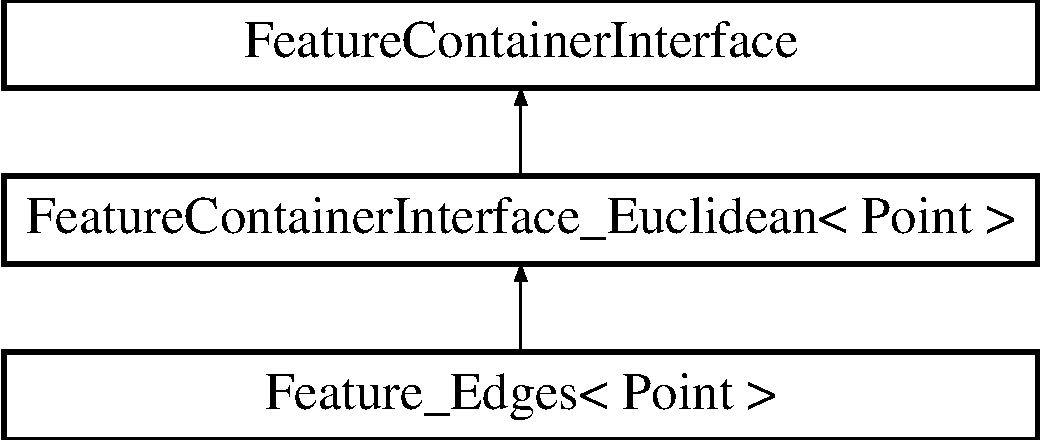
\includegraphics[height=3.000000cm]{classFeature__Edges}
\end{center}
\end{figure}
\subsection*{Public Member Functions}
\begin{DoxyCompactItemize}
\item 
\hypertarget{classFeature__Edges_a41ec56a73dd43ead9c9fe21e7b13dee9}{
void {\bfseries setRadius} (float v)}
\label{classFeature__Edges_a41ec56a73dd43ead9c9fe21e7b13dee9}

\item 
\hypertarget{classFeature__Edges_aa0de4ecd75699f5bf22de8b66b8dcf8f}{
void {\bfseries setThreshold} (float v)}
\label{classFeature__Edges_aa0de4ecd75699f5bf22de8b66b8dcf8f}

\item 
\hypertarget{classFeature__Edges_ab5c0a1152e42c338f0aace02e5e9ed5e}{
void {\bfseries setDisThreshold} (float v)}
\label{classFeature__Edges_ab5c0a1152e42c338f0aace02e5e9ed5e}

\item 
\hypertarget{classFeature__Edges_a81bfa5b7b55f323ee7083aa77b1061a8}{
void {\bfseries extractFeatures} (const pcl::PointCloud$<$ Point $>$ \&point\_\-cloud, pcl::PointCloud$<$ Point $>$ \&narf\_\-descriptors)}
\label{classFeature__Edges_a81bfa5b7b55f323ee7083aa77b1061a8}

\item 
\hypertarget{classFeature__Edges_a9c58dc3da80bde5f40b3c258298c4c3d}{
const pcl::PointCloud$<$ Point $>$ \& {\bfseries getFilteredInputCloud} ()}
\label{classFeature__Edges_a9c58dc3da80bde5f40b3c258298c4c3d}

\item 
\hypertarget{classFeature__Edges_a795dd24e9882c53f3a83ab5bf61d1016}{
const pcl::PointCloud$<$ Point $>$ \& {\bfseries getFilteredOutputCloud} ()}
\label{classFeature__Edges_a795dd24e9882c53f3a83ab5bf61d1016}

\item 
\hypertarget{classFeature__Edges_a10dea841a445f57a5441ecf294b02da7}{
virtual bool {\bfseries hidden\_\-build} ()}
\label{classFeature__Edges_a10dea841a445f57a5441ecf294b02da7}

\item 
\hypertarget{classFeature__Edges_aad4c7a631f08d6a703b52c3d4cafbcf6}{
virtual Eigen::VectorXf {\bfseries getFeatureOut} (const int index)}
\label{classFeature__Edges_aad4c7a631f08d6a703b52c3d4cafbcf6}

\item 
\hypertarget{classFeature__Edges_aeb41e8219b109d0bef79ff9f3206d036}{
virtual Eigen::VectorXf {\bfseries getFeatureIn} (const int index)}
\label{classFeature__Edges_aeb41e8219b109d0bef79ff9f3206d036}

\end{DoxyCompactItemize}
\subsubsection*{template$<$typename Point$>$ class Feature\_\-Edges$<$ Point $>$}



The documentation for this class was generated from the following files:\begin{DoxyCompactItemize}
\item 
common/include/registration/features/edges.h\item 
common/include/registration/features/impl/edges.hpp\end{DoxyCompactItemize}

\hypertarget{classFeature__FPFH}{
\section{Feature\_\-FPFH$<$ Point $>$ Class Template Reference}
\label{classFeature__FPFH}\index{Feature\_\-FPFH@{Feature\_\-FPFH}}
}
Inheritance diagram for Feature\_\-FPFH$<$ Point $>$:\begin{figure}[H]
\begin{center}
\leavevmode
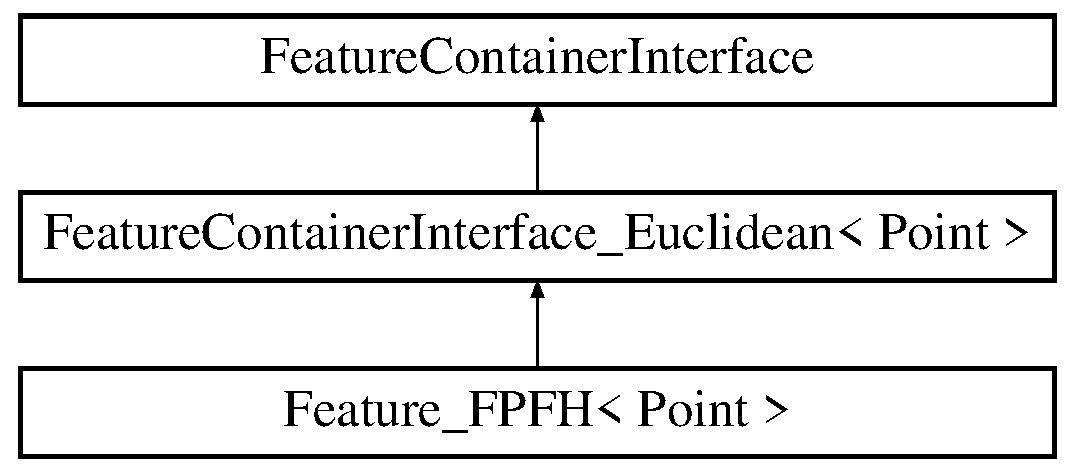
\includegraphics[height=3.000000cm]{classFeature__FPFH}
\end{center}
\end{figure}
\subsection*{Public Member Functions}
\begin{DoxyCompactItemize}
\item 
\hypertarget{classFeature__FPFH_a887dbacf6719f5f3f11cba62296a8ce2}{
void {\bfseries setFPFHRadius} (float v)}
\label{classFeature__FPFH_a887dbacf6719f5f3f11cba62296a8ce2}

\item 
\hypertarget{classFeature__FPFH_a2119fc178835c76d24c2a36a8266e243}{
virtual bool {\bfseries hidden\_\-build} ()}
\label{classFeature__FPFH_a2119fc178835c76d24c2a36a8266e243}

\item 
\hypertarget{classFeature__FPFH_a420b0023c9aff0b4f9dd6a4f6d885279}{
virtual Eigen::VectorXf {\bfseries getFeatureOut} (const int index)}
\label{classFeature__FPFH_a420b0023c9aff0b4f9dd6a4f6d885279}

\item 
\hypertarget{classFeature__FPFH_afab3991e2d23cb74b93a80880c8cd10d}{
virtual Eigen::VectorXf {\bfseries getFeatureIn} (const int index)}
\label{classFeature__FPFH_afab3991e2d23cb74b93a80880c8cd10d}

\end{DoxyCompactItemize}
\subsubsection*{template$<$typename Point$>$ class Feature\_\-FPFH$<$ Point $>$}



The documentation for this class was generated from the following file:\begin{DoxyCompactItemize}
\item 
common/include/registration/features/fast\_\-pfh.h\end{DoxyCompactItemize}

\hypertarget{classFeature__MomentInvariants}{
\section{Feature\_\-MomentInvariants$<$ Point $>$ Class Template Reference}
\label{classFeature__MomentInvariants}\index{Feature\_\-MomentInvariants@{Feature\_\-MomentInvariants}}
}
Inheritance diagram for Feature\_\-MomentInvariants$<$ Point $>$:\begin{figure}[H]
\begin{center}
\leavevmode
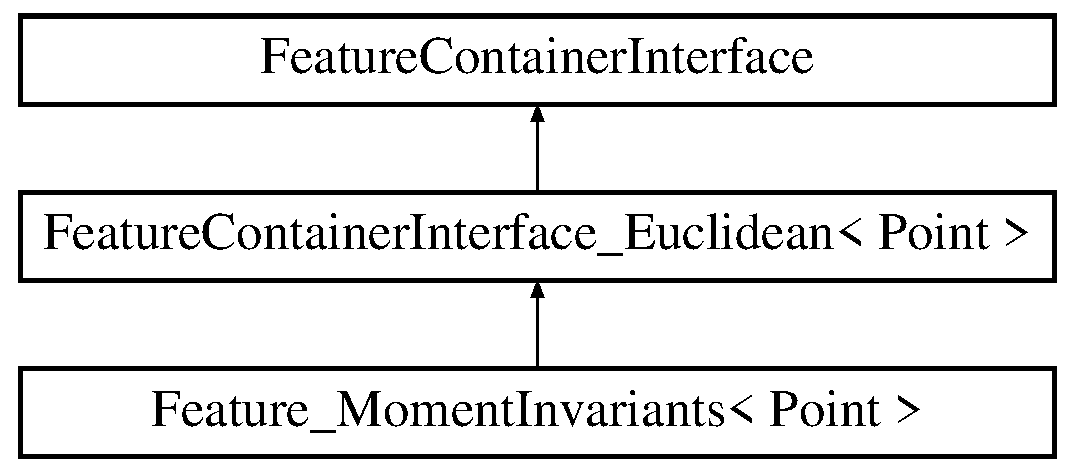
\includegraphics[height=3.000000cm]{classFeature__MomentInvariants}
\end{center}
\end{figure}
\subsection*{Public Member Functions}
\begin{DoxyCompactItemize}
\item 
\hypertarget{classFeature__MomentInvariants_a91c74d851f3da794c382b5e26bb63459}{
void {\bfseries setMomentRadius} (float v)}
\label{classFeature__MomentInvariants_a91c74d851f3da794c382b5e26bb63459}

\item 
\hypertarget{classFeature__MomentInvariants_a813a34ed8a871498bfec8a637345078e}{
virtual bool {\bfseries hidden\_\-build} ()}
\label{classFeature__MomentInvariants_a813a34ed8a871498bfec8a637345078e}

\item 
\hypertarget{classFeature__MomentInvariants_a0a6e40c2a445860db9b8e64807d21e8d}{
virtual Eigen::VectorXf {\bfseries getFeatureOut} (const int index)}
\label{classFeature__MomentInvariants_a0a6e40c2a445860db9b8e64807d21e8d}

\item 
\hypertarget{classFeature__MomentInvariants_a23769a6e06127a376360deae3e405d83}{
virtual Eigen::VectorXf {\bfseries getFeatureIn} (const int index)}
\label{classFeature__MomentInvariants_a23769a6e06127a376360deae3e405d83}

\end{DoxyCompactItemize}
\subsubsection*{template$<$typename Point$>$ class Feature\_\-MomentInvariants$<$ Point $>$}



The documentation for this class was generated from the following file:\begin{DoxyCompactItemize}
\item 
common/include/registration/features/moments.h\end{DoxyCompactItemize}

\hypertarget{classFeature__NARF}{
\section{Feature\_\-NARF$<$ Point $>$ Class Template Reference}
\label{classFeature__NARF}\index{Feature\_\-NARF@{Feature\_\-NARF}}
}
Inheritance diagram for Feature\_\-NARF$<$ Point $>$:\begin{figure}[H]
\begin{center}
\leavevmode
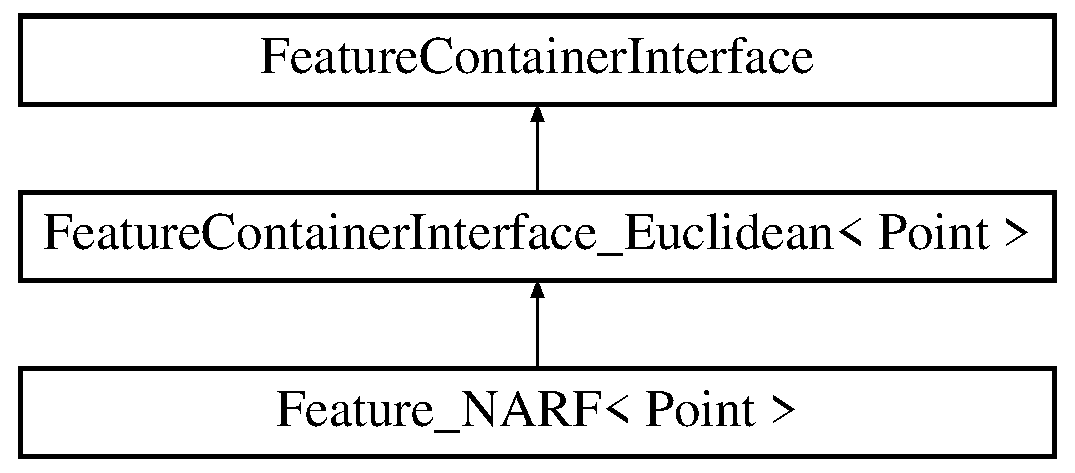
\includegraphics[height=3.000000cm]{classFeature__NARF}
\end{center}
\end{figure}
\subsection*{Public Member Functions}
\begin{DoxyCompactItemize}
\item 
\hypertarget{classFeature__NARF_a70a1a31f0623568e2751159f4655b190}{
const pcl::PointCloud$<$ Point $>$ \& {\bfseries getFilteredInputCloud} ()}
\label{classFeature__NARF_a70a1a31f0623568e2751159f4655b190}

\item 
\hypertarget{classFeature__NARF_ae365ea35195807c992b3876e595247e9}{
const pcl::PointCloud$<$ Point $>$ \& {\bfseries getFilteredOutputCloud} ()}
\label{classFeature__NARF_ae365ea35195807c992b3876e595247e9}

\item 
\hypertarget{classFeature__NARF_ab631be8e4846d2ffd28f957bf645a1a8}{
virtual bool {\bfseries hidden\_\-build} ()}
\label{classFeature__NARF_ab631be8e4846d2ffd28f957bf645a1a8}

\item 
\hypertarget{classFeature__NARF_a61722353ce82ffc97bf05229b08f3bca}{
virtual Eigen::VectorXf {\bfseries getFeatureOut} (const int index)}
\label{classFeature__NARF_a61722353ce82ffc97bf05229b08f3bca}

\item 
\hypertarget{classFeature__NARF_a1aef426f7ba2a31f2011f7d960c9da7b}{
virtual Eigen::VectorXf {\bfseries getFeatureIn} (const int index)}
\label{classFeature__NARF_a1aef426f7ba2a31f2011f7d960c9da7b}

\end{DoxyCompactItemize}
\subsection*{Static Public Member Functions}
\begin{DoxyCompactItemize}
\item 
\hypertarget{classFeature__NARF_a472d7f903789b0c828f03f25fb0f6acc}{
static void {\bfseries extractFeatures} (const pcl::PointCloud$<$ Point $>$ \&point\_\-cloud, pcl::PointCloud$<$ pcl::Narf36 $>$ \&narf\_\-descriptors)}
\label{classFeature__NARF_a472d7f903789b0c828f03f25fb0f6acc}

\end{DoxyCompactItemize}
\subsubsection*{template$<$typename Point$>$ class Feature\_\-NARF$<$ Point $>$}



The documentation for this class was generated from the following files:\begin{DoxyCompactItemize}
\item 
common/include/registration/features/narf.h\item 
common/include/registration/features/impl/narf.hpp\end{DoxyCompactItemize}

\hypertarget{classFeatureContainer}{
\section{FeatureContainer$<$ FeatureType $>$ Class Template Reference}
\label{classFeatureContainer}\index{FeatureContainer@{FeatureContainer}}
}
Inheritance diagram for FeatureContainer$<$ FeatureType $>$:\begin{figure}[H]
\begin{center}
\leavevmode
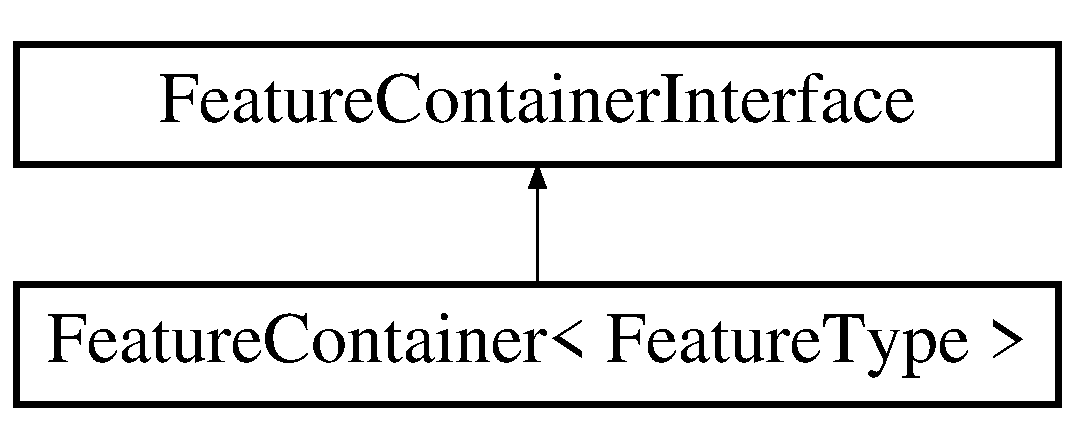
\includegraphics[height=2.000000cm]{classFeatureContainer}
\end{center}
\end{figure}
\subsection*{Public Types}
\begin{DoxyCompactItemize}
\item 
\hypertarget{classFeatureContainer_a812a7f7cfef2ac98ddc5e2483de4fd20}{
typedef pcl::PointCloud$<$ FeatureType $>$::ConstPtr {\bfseries FeatureCloudConstPtr}}
\label{classFeatureContainer_a812a7f7cfef2ac98ddc5e2483de4fd20}

\item 
\hypertarget{classFeatureContainer_aa9b344b371c9e07ff390d1628dfbcaf4}{
typedef pcl::KdTree$<$ FeatureType $>$ {\bfseries KdTree}}
\label{classFeatureContainer_aa9b344b371c9e07ff390d1628dfbcaf4}

\item 
\hypertarget{classFeatureContainer_a4c74fecce5bc9b613831e10c8027da9b}{
typedef pcl::KdTree$<$ FeatureType $>$::Ptr {\bfseries KdTreePtr}}
\label{classFeatureContainer_a4c74fecce5bc9b613831e10c8027da9b}

\item 
\hypertarget{classFeatureContainer_ae50b6e9fde0e0c2533a18f905bb963de}{
typedef boost::function$<$ int(const pcl::PointCloud$<$ FeatureType $>$ \&, int, std::vector$<$ int $>$ \&, std::vector$<$ float $>$ \&)$>$ {\bfseries SearchMethod}}
\label{classFeatureContainer_ae50b6e9fde0e0c2533a18f905bb963de}

\end{DoxyCompactItemize}
\subsection*{Public Member Functions}
\begin{DoxyCompactItemize}
\item 
\hypertarget{classFeatureContainer_a25bae377554ca46d3ceeb0e75b94a1df}{
void {\bfseries setSourceFeature} (const FeatureCloudConstPtr \&source\_\-features)}
\label{classFeatureContainer_a25bae377554ca46d3ceeb0e75b94a1df}

\item 
\hypertarget{classFeatureContainer_ae60b59ddad5f99c33976dacc8f51313f}{
FeatureCloudConstPtr {\bfseries getSourceFeature} ()}
\label{classFeatureContainer_ae60b59ddad5f99c33976dacc8f51313f}

\item 
\hypertarget{classFeatureContainer_a9b33939542a0e0a44ea929fa94144fd0}{
void {\bfseries setTargetFeature} (const FeatureCloudConstPtr \&target\_\-features)}
\label{classFeatureContainer_a9b33939542a0e0a44ea929fa94144fd0}

\item 
\hypertarget{classFeatureContainer_a6b9b90e2d4c0cffa66a6aad566a5398b}{
FeatureCloudConstPtr {\bfseries getTargetFeature} ()}
\label{classFeatureContainer_a6b9b90e2d4c0cffa66a6aad566a5398b}

\item 
\hypertarget{classFeatureContainer_afba51926e3b8f1469f2056c3a0e67233}{
void {\bfseries setRadiusSearch} (KdTreePtr tree, float r)}
\label{classFeatureContainer_afba51926e3b8f1469f2056c3a0e67233}

\item 
\hypertarget{classFeatureContainer_a5eb230cc0dae19264e37004cd77f0084}{
void {\bfseries setKSearch} (KdTreePtr tree, int k)}
\label{classFeatureContainer_a5eb230cc0dae19264e37004cd77f0084}

\item 
\hypertarget{classFeatureContainer_a42bd311329ec0278af0f744cbbf224ef}{
virtual bool {\bfseries isValid} ()}
\label{classFeatureContainer_a42bd311329ec0278af0f744cbbf224ef}

\item 
\hypertarget{classFeatureContainer_a666fa9a8410848c218a816680704e846}{
virtual void {\bfseries findFeatureCorrespondences} (int index, std::vector$<$ int $>$ \&correspondence\_\-indices, std::vector$<$ float $>$ \&distances)}
\label{classFeatureContainer_a666fa9a8410848c218a816680704e846}

\end{DoxyCompactItemize}
\subsubsection*{template$<$typename FeatureType$>$ class FeatureContainer$<$ FeatureType $>$}



The documentation for this class was generated from the following file:\begin{DoxyCompactItemize}
\item 
common/include/registration/feature\_\-container.h\end{DoxyCompactItemize}

\hypertarget{classFeatureContainerInterface}{
\section{FeatureContainerInterface Class Reference}
\label{classFeatureContainerInterface}\index{FeatureContainerInterface@{FeatureContainerInterface}}
}
Inheritance diagram for FeatureContainerInterface:\begin{figure}[H]
\begin{center}
\leavevmode
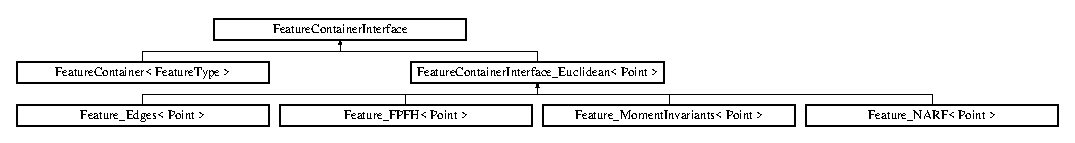
\includegraphics[height=1.478873cm]{classFeatureContainerInterface}
\end{center}
\end{figure}
\subsection*{Public Member Functions}
\begin{DoxyCompactItemize}
\item 
\hypertarget{classFeatureContainerInterface_a9568589d47d1d10cfb86994b0447b929}{
virtual bool {\bfseries isValid} ()=0}
\label{classFeatureContainerInterface_a9568589d47d1d10cfb86994b0447b929}

\item 
\hypertarget{classFeatureContainerInterface_a0f2f617c6a7b3550ede10ff9c119dbaf}{
virtual void {\bfseries findFeatureCorrespondences} (int index, std::vector$<$ int $>$ \&correspondence\_\-indices, std::vector$<$ float $>$ \&distances)=0}
\label{classFeatureContainerInterface_a0f2f617c6a7b3550ede10ff9c119dbaf}

\end{DoxyCompactItemize}


The documentation for this class was generated from the following file:\begin{DoxyCompactItemize}
\item 
common/include/registration/feature\_\-container.h\end{DoxyCompactItemize}

\hypertarget{classFeatureContainerInterface__Euclidean}{
\section{FeatureContainerInterface\_\-Euclidean$<$ Point $>$ Class Template Reference}
\label{classFeatureContainerInterface__Euclidean}\index{FeatureContainerInterface\_\-Euclidean@{FeatureContainerInterface\_\-Euclidean}}
}
Inheritance diagram for FeatureContainerInterface\_\-Euclidean$<$ Point $>$:\begin{figure}[H]
\begin{center}
\leavevmode
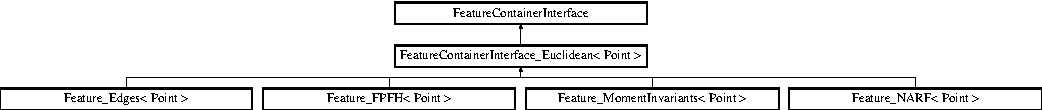
\includegraphics[height=1.478873cm]{classFeatureContainerInterface__Euclidean}
\end{center}
\end{figure}
\subsection*{Public Member Functions}
\begin{DoxyCompactItemize}
\item 
\hypertarget{classFeatureContainerInterface__Euclidean_ae494f98d4348890e446968219fa0378a}{
void {\bfseries setSearchRadius} (float v)}
\label{classFeatureContainerInterface__Euclidean_ae494f98d4348890e446968219fa0378a}

\item 
\hypertarget{classFeatureContainerInterface__Euclidean_a950d53fcc1a629d6a39e43d0dba1bea9}{
virtual void {\bfseries build} (const pcl::PointCloud$<$ Point $>$ \&src, const pcl::PointCloud$<$ Point $>$ \&tgt)}
\label{classFeatureContainerInterface__Euclidean_a950d53fcc1a629d6a39e43d0dba1bea9}

\item 
\hypertarget{classFeatureContainerInterface__Euclidean_a569e4e9d4d5d7fb47121b1817bf91317}{
virtual bool {\bfseries isValid} ()}
\label{classFeatureContainerInterface__Euclidean_a569e4e9d4d5d7fb47121b1817bf91317}

\item 
\hypertarget{classFeatureContainerInterface__Euclidean_a4b5f71d89551a4df0a43daa8ce95e51f}{
virtual void {\bfseries findFeatureCorrespondences} (int index, std::vector$<$ int $>$ \&correspondence\_\-indices, std::vector$<$ float $>$ \&distances)}
\label{classFeatureContainerInterface__Euclidean_a4b5f71d89551a4df0a43daa8ce95e51f}

\item 
\hypertarget{classFeatureContainerInterface__Euclidean_ad4fc430a94ee6c06bc1887e413af4009}{
virtual Eigen::VectorXf {\bfseries getFeatureOut} (const int)=0}
\label{classFeatureContainerInterface__Euclidean_ad4fc430a94ee6c06bc1887e413af4009}

\item 
\hypertarget{classFeatureContainerInterface__Euclidean_a873f51708a90edd5b01de5a86e81cdb0}{
virtual Eigen::VectorXf {\bfseries getFeatureIn} (const int)=0}
\label{classFeatureContainerInterface__Euclidean_a873f51708a90edd5b01de5a86e81cdb0}

\item 
\hypertarget{classFeatureContainerInterface__Euclidean_af8f2128c44deec743d0ede1cc40d83fc}{
virtual bool {\bfseries hidden\_\-build} ()=0}
\label{classFeatureContainerInterface__Euclidean_af8f2128c44deec743d0ede1cc40d83fc}

\end{DoxyCompactItemize}
\subsection*{Protected Attributes}
\begin{DoxyCompactItemize}
\item 
\hypertarget{classFeatureContainerInterface__Euclidean_a3cdddedc9eaffa1904130e44b1991837}{
bool {\bfseries build\_\-}}
\label{classFeatureContainerInterface__Euclidean_a3cdddedc9eaffa1904130e44b1991837}

\item 
\hypertarget{classFeatureContainerInterface__Euclidean_a911fef526cc7c6e25e0fd3a301cbd09b}{
float {\bfseries radius2\_\-}}
\label{classFeatureContainerInterface__Euclidean_a911fef526cc7c6e25e0fd3a301cbd09b}

\item 
\hypertarget{classFeatureContainerInterface__Euclidean_a0f447e12451abb8eb49fcf574758f588}{
pcl::PointCloud$<$ Point $>$ {\bfseries org\_\-in\_\-}}
\label{classFeatureContainerInterface__Euclidean_a0f447e12451abb8eb49fcf574758f588}

\item 
\hypertarget{classFeatureContainerInterface__Euclidean_abac547071ead25c6c676b56a2d5dee20}{
pcl::PointCloud$<$ Point $>$ {\bfseries org\_\-out\_\-}}
\label{classFeatureContainerInterface__Euclidean_abac547071ead25c6c676b56a2d5dee20}

\item 
\hypertarget{classFeatureContainerInterface__Euclidean_a283c12b73d04f8d5fe2e2a3d04d1b7a1}{
boost::shared\_\-ptr$<$ pcl::KdTree$<$ Point $>$ $>$ {\bfseries tree\_\-}}
\label{classFeatureContainerInterface__Euclidean_a283c12b73d04f8d5fe2e2a3d04d1b7a1}

\end{DoxyCompactItemize}
\subsubsection*{template$<$typename Point$>$ class FeatureContainerInterface\_\-Euclidean$<$ Point $>$}



The documentation for this class was generated from the following file:\begin{DoxyCompactItemize}
\item 
common/include/registration/feature\_\-container.h\end{DoxyCompactItemize}

\hypertarget{classFilterNode}{
\section{FilterNode Class Reference}
\label{classFilterNode}\index{FilterNode@{FilterNode}}
}
\subsection*{Public Member Functions}
\begin{DoxyCompactItemize}
\item 
void \hyperlink{classFilterNode_ad5a6037efebea20a732786f22b3d57c8}{onInit} ()
\begin{DoxyCompactList}\small\item\em initializes parameters \item\end{DoxyCompactList}\item 
void \hyperlink{classFilterNode_aa2a751b356c5e5d526176a039593c53a}{pointCloudSubCallback} (const pcl::PointCloud$<$ Point $>$::Ptr \&pc\_\-in)
\begin{DoxyCompactList}\small\item\em callback for point cloud subroutine \item\end{DoxyCompactList}\item 
\hypertarget{classFilterNode_a8c503939ad8cd17f44ac0eca14b8bb70}{
bool {\bfseries filterService} (registration::RegistrationPCD::Request \&req, registration::RegistrationPCD::Response \&res)}
\label{classFilterNode_a8c503939ad8cd17f44ac0eca14b8bb70}

\end{DoxyCompactItemize}
\subsection*{Public Attributes}
\begin{DoxyCompactItemize}
\item 
\hypertarget{classFilterNode_a25e814d44b3b82d31110b5d38ebae9ab}{
ros::NodeHandle {\bfseries n\_\-}}
\label{classFilterNode_a25e814d44b3b82d31110b5d38ebae9ab}

\item 
\hypertarget{classFilterNode_a534f1ee93b0ef514ba610077791b8bdf}{
ros::Time {\bfseries stamp\_\-}}
\label{classFilterNode_a534f1ee93b0ef514ba610077791b8bdf}

\end{DoxyCompactItemize}
\subsection*{Protected Attributes}
\begin{DoxyCompactItemize}
\item 
\hypertarget{classFilterNode_a8c5df30549e5e51af6c78b0e9e4291c0}{
ros::Subscriber {\bfseries point\_\-cloud\_\-sub\_\-}}
\label{classFilterNode_a8c5df30549e5e51af6c78b0e9e4291c0}

\item 
\hypertarget{classFilterNode_a81a73041da925168f59ca5d59324585b}{
ros::Publisher {\bfseries point\_\-cloud\_\-pub\_\-}}
\label{classFilterNode_a81a73041da925168f59ca5d59324585b}

\item 
\hypertarget{classFilterNode_ac4cde7e6324564c25c5c184ee781cfe8}{
ros::ServiceServer {\bfseries filter\_\-ser\_\-}}
\label{classFilterNode_ac4cde7e6324564c25c5c184ee781cfe8}

\end{DoxyCompactItemize}


\subsection{Member Function Documentation}
\hypertarget{classFilterNode_ad5a6037efebea20a732786f22b3d57c8}{
\index{FilterNode@{FilterNode}!onInit@{onInit}}
\index{onInit@{onInit}!FilterNode@{FilterNode}}
\subsubsection[{onInit}]{\setlength{\rightskip}{0pt plus 5cm}void FilterNode::onInit (
\begin{DoxyParamCaption}
{}
\end{DoxyParamCaption}
)\hspace{0.3cm}{\ttfamily  \mbox{[}inline\mbox{]}}}}
\label{classFilterNode_ad5a6037efebea20a732786f22b3d57c8}


initializes parameters 

initializes parameters

\begin{DoxyReturn}{Returns}
nothing 
\end{DoxyReturn}
\hypertarget{classFilterNode_aa2a751b356c5e5d526176a039593c53a}{
\index{FilterNode@{FilterNode}!pointCloudSubCallback@{pointCloudSubCallback}}
\index{pointCloudSubCallback@{pointCloudSubCallback}!FilterNode@{FilterNode}}
\subsubsection[{pointCloudSubCallback}]{\setlength{\rightskip}{0pt plus 5cm}void FilterNode::pointCloudSubCallback (
\begin{DoxyParamCaption}
\item[{const pcl::PointCloud$<$ Point $>$::Ptr \&}]{ pc\_\-in}
\end{DoxyParamCaption}
)\hspace{0.3cm}{\ttfamily  \mbox{[}inline\mbox{]}}}}
\label{classFilterNode_aa2a751b356c5e5d526176a039593c53a}


callback for point cloud subroutine 

callback for point cloud subroutine which stores the point cloud for further calculation


\begin{DoxyParams}{Parameters}
\item[{\em pc\_\-in}]new point cloud\end{DoxyParams}
\begin{DoxyReturn}{Returns}
nothing 
\end{DoxyReturn}


The documentation for this class was generated from the following file:\begin{DoxyCompactItemize}
\item 
ros/src/filter.cpp\end{DoxyCompactItemize}

\hypertarget{classGeneralRegistration}{
\section{GeneralRegistration$<$ Point $>$ Class Template Reference}
\label{classGeneralRegistration}\index{GeneralRegistration@{GeneralRegistration}}
}


{\ttfamily \#include $<$general\_\-registration.h$>$}

Inheritance diagram for GeneralRegistration$<$ Point $>$:\begin{figure}[H]
\begin{center}
\leavevmode
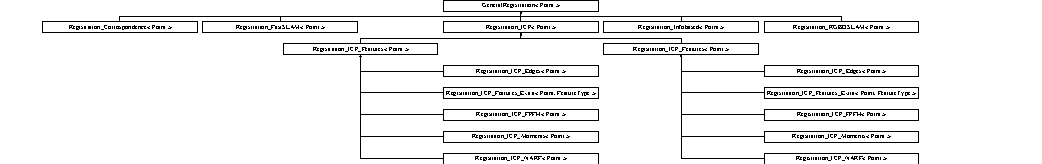
\includegraphics[height=2.202557cm]{classGeneralRegistration}
\end{center}
\end{figure}
\subsection*{Public Member Functions}
\begin{DoxyCompactItemize}
\item 
\hypertarget{classGeneralRegistration_a13eb99cd3da37c3bea5c0f0804eb464c}{
virtual void \hyperlink{classGeneralRegistration_a13eb99cd3da37c3bea5c0f0804eb464c}{setOdometry} (const Eigen::Matrix4f \&odometry)}
\label{classGeneralRegistration_a13eb99cd3da37c3bea5c0f0804eb464c}

\begin{DoxyCompactList}\small\item\em change transformation matrix (for example if odometry results are known) \item\end{DoxyCompactList}\item 
\hypertarget{classGeneralRegistration_ac4d5bfb0b8e14945ec99708093e63bd7}{
virtual void \hyperlink{classGeneralRegistration_ac4d5bfb0b8e14945ec99708093e63bd7}{setInputCloud} (const boost::shared\_\-ptr$<$ const pcl::PointCloud$<$ Point $>$ $>$ \&cloud)}
\label{classGeneralRegistration_ac4d5bfb0b8e14945ec99708093e63bd7}

\begin{DoxyCompactList}\small\item\em sets preprocessed input cloud \item\end{DoxyCompactList}\item 
\hypertarget{classGeneralRegistration_a8bd91517840e7a1b075814944ae34451}{
virtual void \hyperlink{classGeneralRegistration_a8bd91517840e7a1b075814944ae34451}{setInputOginalCloud} (const boost::shared\_\-ptr$<$ const pcl::PointCloud$<$ Point $>$ $>$ \&cloud)}
\label{classGeneralRegistration_a8bd91517840e7a1b075814944ae34451}

\begin{DoxyCompactList}\small\item\em sets orginal input cloud \item\end{DoxyCompactList}\item 
\hypertarget{classGeneralRegistration_a627f43f8f614954e66a0328dbd7ea539}{
virtual void \hyperlink{classGeneralRegistration_a627f43f8f614954e66a0328dbd7ea539}{setInputImage} (const boost::shared\_\-ptr$<$ const cv::Mat $>$ \&img)}
\label{classGeneralRegistration_a627f43f8f614954e66a0328dbd7ea539}

\begin{DoxyCompactList}\small\item\em set color image \item\end{DoxyCompactList}\item 
\hypertarget{classGeneralRegistration_a9302c8dbf62533851ef2f9ca888dcc7a}{
virtual void \hyperlink{classGeneralRegistration_a9302c8dbf62533851ef2f9ca888dcc7a}{setInputDepthImage} (const boost::shared\_\-ptr$<$ const cv::Mat $>$ \&img)}
\label{classGeneralRegistration_a9302c8dbf62533851ef2f9ca888dcc7a}

\begin{DoxyCompactList}\small\item\em set disparity image \item\end{DoxyCompactList}\item 
\hypertarget{classGeneralRegistration_aeeaa5ccc625af76c73fd95165447ca61}{
virtual boost::shared\_\-ptr$<$ const pcl::PointCloud$<$ Point $>$ $>$ \hyperlink{classGeneralRegistration_aeeaa5ccc625af76c73fd95165447ca61}{getMarkers} ()}
\label{classGeneralRegistration_aeeaa5ccc625af76c73fd95165447ca61}

\begin{DoxyCompactList}\small\item\em debug function for marker visualization \item\end{DoxyCompactList}\item 
virtual bool \hyperlink{classGeneralRegistration_a1576d568bd1bc5de026be9441eeabd48}{compute} ()
\item 
\hypertarget{classGeneralRegistration_acb98af3d4fce5549db0c3fd7fb880c07}{
virtual Eigen::Matrix4f \hyperlink{classGeneralRegistration_acb98af3d4fce5549db0c3fd7fb880c07}{getTransformation} () const }
\label{classGeneralRegistration_acb98af3d4fce5549db0c3fd7fb880c07}

\begin{DoxyCompactList}\small\item\em get transformation \item\end{DoxyCompactList}\item 
\hypertarget{classGeneralRegistration_aa3ecd55d2f293a224049ca47be3a07c8}{
virtual boost::shared\_\-ptr$<$ pcl::PointCloud$<$ Point $>$ $>$ \hyperlink{classGeneralRegistration_aa3ecd55d2f293a224049ca47be3a07c8}{getMap} ()}
\label{classGeneralRegistration_aa3ecd55d2f293a224049ca47be3a07c8}

\begin{DoxyCompactList}\small\item\em map is not necessarily implemented \item\end{DoxyCompactList}\end{DoxyCompactItemize}
\subsection*{Protected Member Functions}
\begin{DoxyCompactItemize}
\item 
\hypertarget{classGeneralRegistration_a94d7c0dd8543687ae9e8421ac748aa4f}{
virtual bool {\bfseries compute\_\-features} ()=0}
\label{classGeneralRegistration_a94d7c0dd8543687ae9e8421ac748aa4f}

\item 
\hypertarget{classGeneralRegistration_aa2fc4bfbc908fd44b1eed39bab026e15}{
virtual bool {\bfseries compute\_\-corrospondences} ()=0}
\label{classGeneralRegistration_aa2fc4bfbc908fd44b1eed39bab026e15}

\item 
\hypertarget{classGeneralRegistration_a689e345417d73a82f1bf7d500b5805c4}{
virtual bool {\bfseries compute\_\-transformation} ()=0}
\label{classGeneralRegistration_a689e345417d73a82f1bf7d500b5805c4}

\end{DoxyCompactItemize}
\subsection*{Protected Attributes}
\begin{DoxyCompactItemize}
\item 
\hypertarget{classGeneralRegistration_ab4dc735822c32d0496aa7b84e845bf29}{
boost::shared\_\-ptr$<$ const pcl::PointCloud$<$ Point $>$ $>$ {\bfseries input\_\-}}
\label{classGeneralRegistration_ab4dc735822c32d0496aa7b84e845bf29}

\item 
\hypertarget{classGeneralRegistration_a82b4489bc709fd88197929f0a450c95d}{
boost::shared\_\-ptr$<$ const pcl::PointCloud$<$ Point $>$ $>$ {\bfseries input\_\-org\_\-}}
\label{classGeneralRegistration_a82b4489bc709fd88197929f0a450c95d}

\item 
\hypertarget{classGeneralRegistration_ad2933061cf77cdca3ae2df27048414c6}{
boost::shared\_\-ptr$<$ const cv::Mat $>$ {\bfseries input\_\-image\_\-}}
\label{classGeneralRegistration_ad2933061cf77cdca3ae2df27048414c6}

\item 
\hypertarget{classGeneralRegistration_acb62a0b225a3c4fdb6e22696156a249f}{
boost::shared\_\-ptr$<$ const cv::Mat $>$ {\bfseries input\_\-depth\_\-image\_\-}}
\label{classGeneralRegistration_acb62a0b225a3c4fdb6e22696156a249f}

\item 
\hypertarget{classGeneralRegistration_a6cbc0cdb17ce37dab567abce1aad3d2c}{
Eigen::Matrix4f {\bfseries transformation\_\-}}
\label{classGeneralRegistration_a6cbc0cdb17ce37dab567abce1aad3d2c}

\end{DoxyCompactItemize}


\subsection{Detailed Description}
\subsubsection*{template$<$typename Point$>$ class GeneralRegistration$<$ Point $>$}

a general abstract class for registration purpose of 3d pointclouds as input it's espected to provide ...
\begin{DoxyItemize}
\item the original (dense) pointcloud
\item the preprocessed pointcloud
\item the color image
\item the depth image not all of the input data are necessary to all registration methods if you are in need to spare one or more please refer to the used algorithms result of compute is the success status and the transformation 
\end{DoxyItemize}

\subsection{Member Function Documentation}
\hypertarget{classGeneralRegistration_a1576d568bd1bc5de026be9441eeabd48}{
\index{GeneralRegistration@{GeneralRegistration}!compute@{compute}}
\index{compute@{compute}!GeneralRegistration@{GeneralRegistration}}
\subsubsection[{compute}]{\setlength{\rightskip}{0pt plus 5cm}template$<$typename Point $>$ virtual bool {\bf GeneralRegistration}$<$ Point $>$::compute (
\begin{DoxyParamCaption}
{}
\end{DoxyParamCaption}
)\hspace{0.3cm}{\ttfamily  \mbox{[}inline, virtual\mbox{]}}}}
\label{classGeneralRegistration_a1576d568bd1bc5de026be9441eeabd48}
compute transformation \begin{DoxyReturn}{Returns}
true for success 
\end{DoxyReturn}


The documentation for this class was generated from the following file:\begin{DoxyCompactItemize}
\item 
common/include/registration/general\_\-registration.h\end{DoxyCompactItemize}

\hypertarget{classGeneralSLAM_3_01Point_01_4}{
\section{GeneralSLAM$<$ Point $>$ Class Template Reference}
\label{classGeneralSLAM_3_01Point_01_4}\index{GeneralSLAM$<$ Point $>$@{GeneralSLAM$<$ Point $>$}}
}
\subsection*{Public Member Functions}
\begin{DoxyCompactItemize}
\item 
\hypertarget{classGeneralSLAM_3_01Point_01_4_ad5e6253055dbce078237df09ca214f7f}{
virtual void {\bfseries setInputCloud} (const PointCloudConstPtr \&cloud)}
\label{classGeneralSLAM_3_01Point_01_4_ad5e6253055dbce078237df09ca214f7f}

\item 
\hypertarget{classGeneralSLAM_3_01Point_01_4_a933a894a635bec386c52d419c6fe6eaf}{
virtual void {\bfseries setOdometry} (const Eigen::Matrix4f \&odometry)}
\label{classGeneralSLAM_3_01Point_01_4_a933a894a635bec386c52d419c6fe6eaf}

\item 
\hypertarget{classGeneralSLAM_3_01Point_01_4_a4e88110d75d7ef1e4f66b10e3c746e4b}{
virtual pcl::PointCloud$<$ Point $>$::ConstPtr {\bfseries getMap} ()}
\label{classGeneralSLAM_3_01Point_01_4_a4e88110d75d7ef1e4f66b10e3c746e4b}

\item 
\hypertarget{classGeneralSLAM_3_01Point_01_4_a388cf32bdea9d6ef0f65a2cbe1ff50ed}{
virtual bool {\bfseries compute} ()}
\label{classGeneralSLAM_3_01Point_01_4_a388cf32bdea9d6ef0f65a2cbe1ff50ed}

\end{DoxyCompactItemize}
\subsection*{Protected Member Functions}
\begin{DoxyCompactItemize}
\item 
\hypertarget{classGeneralSLAM_3_01Point_01_4_abe93ad9710699113fb3e592c4d99b3bc}{
virtual bool {\bfseries compute\_\-registration} ()=0}
\label{classGeneralSLAM_3_01Point_01_4_abe93ad9710699113fb3e592c4d99b3bc}

\item 
\hypertarget{classGeneralSLAM_3_01Point_01_4_a17daec21ee9f79c09b045f3d8bf61c5b}{
virtual bool {\bfseries compute\_\-transformation} ()=0}
\label{classGeneralSLAM_3_01Point_01_4_a17daec21ee9f79c09b045f3d8bf61c5b}

\item 
\hypertarget{classGeneralSLAM_3_01Point_01_4_a0025a4dc5d69ae918fb55a0c6a74b4f6}{
virtual bool {\bfseries compute\_\-map} ()=0}
\label{classGeneralSLAM_3_01Point_01_4_a0025a4dc5d69ae918fb55a0c6a74b4f6}

\end{DoxyCompactItemize}
\subsection*{Protected Attributes}
\begin{DoxyCompactItemize}
\item 
\hypertarget{classGeneralSLAM_3_01Point_01_4_a250138ef64661c18894c16ed142b7d5f}{
PointCloudConstPtr {\bfseries input\_\-}}
\label{classGeneralSLAM_3_01Point_01_4_a250138ef64661c18894c16ed142b7d5f}

\item 
\hypertarget{classGeneralSLAM_3_01Point_01_4_a5b4fe56676045b85659fc8498ef06d66}{
pcl::PointCloud$<$ Point $>$ {\bfseries map\_\-}}
\label{classGeneralSLAM_3_01Point_01_4_a5b4fe56676045b85659fc8498ef06d66}

\item 
\hypertarget{classGeneralSLAM_3_01Point_01_4_a24025bdd56359ca77b79bc28b8412264}{
Eigen::Matrix4f {\bfseries odometry\_\-}}
\label{classGeneralSLAM_3_01Point_01_4_a24025bdd56359ca77b79bc28b8412264}

\end{DoxyCompactItemize}
\subsubsection*{template$<$class Point$>$ class GeneralSLAM$<$ Point $>$}



The documentation for this class was generated from the following file:\begin{DoxyCompactItemize}
\item 
common/include/registration/general\_\-slam.hpp\end{DoxyCompactItemize}

\hypertarget{classpcl_1_1IterativeClosestPoint}{
\section{IterativeClosestPoint Class Reference}
\label{classpcl_1_1IterativeClosestPoint}\index{pcl::IterativeClosestPoint@{pcl::IterativeClosestPoint}}
}
Inheritance diagram for IterativeClosestPoint:\begin{figure}[H]
\begin{center}
\leavevmode
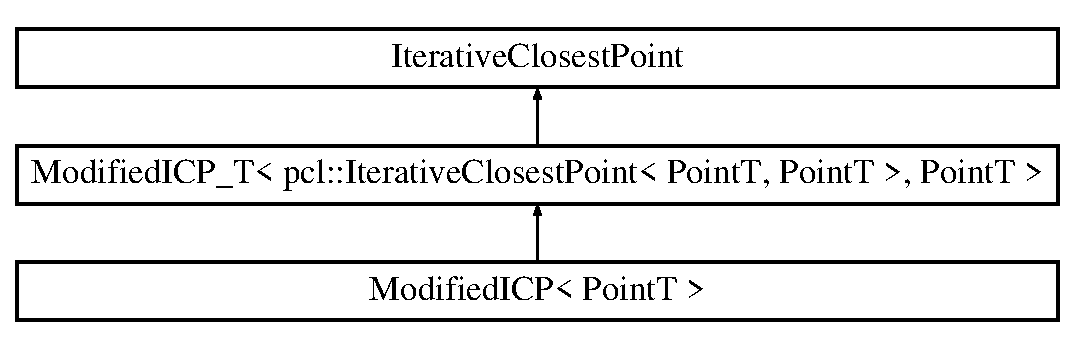
\includegraphics[height=3.000000cm]{classpcl_1_1IterativeClosestPoint}
\end{center}
\end{figure}


The documentation for this class was generated from the following file:\begin{DoxyCompactItemize}
\item 
common/include/registration/impl/modified\_\-icp.hpp\end{DoxyCompactItemize}

\hypertarget{classKeypoints__Narf}{
\section{Keypoints\_\-Narf$<$ Point $>$ Class Template Reference}
\label{classKeypoints__Narf}\index{Keypoints\_\-Narf@{Keypoints\_\-Narf}}
}
Inheritance diagram for Keypoints\_\-Narf$<$ Point $>$:\begin{figure}[H]
\begin{center}
\leavevmode
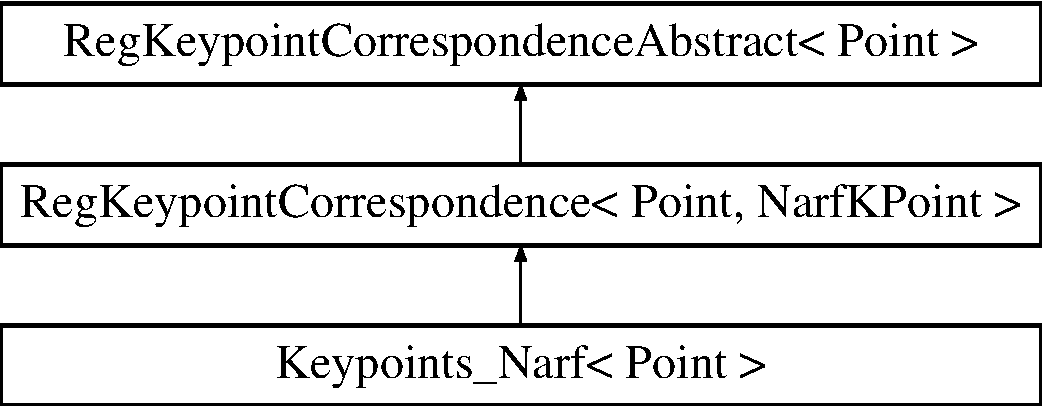
\includegraphics[height=3.000000cm]{classKeypoints__Narf}
\end{center}
\end{figure}
\subsection*{Public Member Functions}
\begin{DoxyCompactItemize}
\item 
\hypertarget{classKeypoints__Narf_a43abbb08515b95bab17c0da74e6f8575}{
void {\bfseries setRadius} (float v)}
\label{classKeypoints__Narf_a43abbb08515b95bab17c0da74e6f8575}

\item 
\hypertarget{classKeypoints__Narf_aa52165facc800efa865888b608c7a558}{
void {\bfseries setThreshold} (float v)}
\label{classKeypoints__Narf_aa52165facc800efa865888b608c7a558}

\item 
\hypertarget{classKeypoints__Narf_a7476a84609be6d463d32234576387863}{
void {\bfseries setDisThreshold} (float v)}
\label{classKeypoints__Narf_a7476a84609be6d463d32234576387863}

\item 
\hypertarget{classKeypoints__Narf_a156b9ccd8faae2612e57a92163bf416c}{
virtual bool {\bfseries compute} (const pcl::PointCloud$<$ Point $>$ \&src, const pcl::PointCloud$<$ Point $>$ \&tgt)}
\label{classKeypoints__Narf_a156b9ccd8faae2612e57a92163bf416c}

\item 
\hypertarget{classKeypoints__Narf_aa975bf558ca1d1e5a7f0ebeca2cfb309}{
virtual void {\bfseries getCorrespondences} (std::vector$<$ pcl::registration::Correspondence $>$ \&correspondences)}
\label{classKeypoints__Narf_aa975bf558ca1d1e5a7f0ebeca2cfb309}

\item 
\hypertarget{classKeypoints__Narf_a7e02a9e934786fa9c16f686b6dda77c6}{
Point {\bfseries getPointForKeypointSrc} (const int ind)}
\label{classKeypoints__Narf_a7e02a9e934786fa9c16f686b6dda77c6}

\item 
\hypertarget{classKeypoints__Narf_a3c1880248904e955009daf55314c3fa7}{
Point {\bfseries getPointForKeypointTgt} (const int ind)}
\label{classKeypoints__Narf_a3c1880248904e955009daf55314c3fa7}

\end{DoxyCompactItemize}
\subsubsection*{template$<$typename Point$>$ class Keypoints\_\-Narf$<$ Point $>$}



The documentation for this class was generated from the following files:\begin{DoxyCompactItemize}
\item 
common/include/registration/features/narf\_\-kp.h\item 
common/include/registration/features/impl/narf\_\-kp.hpp\end{DoxyCompactItemize}

\hypertarget{classKeypoints__Segments}{
\section{Keypoints\_\-Segments$<$ Point $>$ Class Template Reference}
\label{classKeypoints__Segments}\index{Keypoints\_\-Segments@{Keypoints\_\-Segments}}
}
Inheritance diagram for Keypoints\_\-Segments$<$ Point $>$:\begin{figure}[H]
\begin{center}
\leavevmode
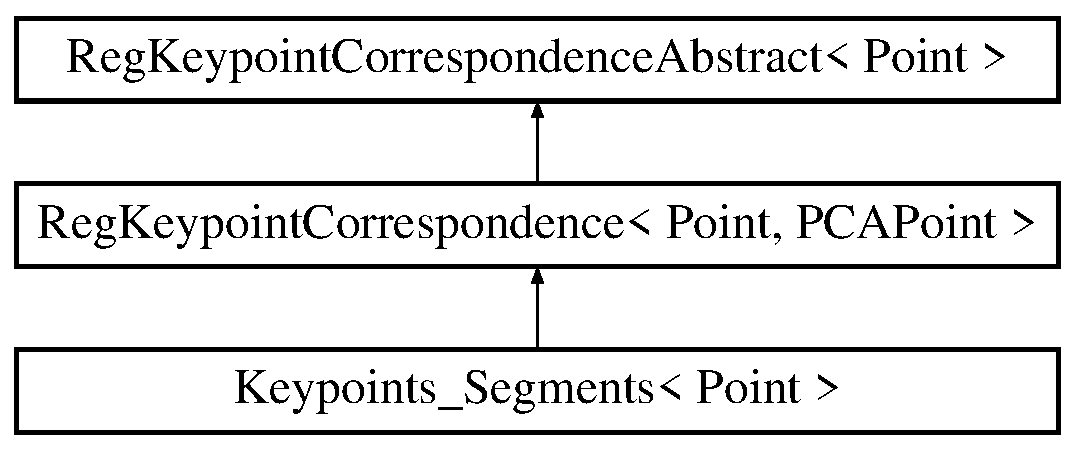
\includegraphics[height=3.000000cm]{classKeypoints__Segments}
\end{center}
\end{figure}
\subsection*{Public Member Functions}
\begin{DoxyCompactItemize}
\item 
\hypertarget{classKeypoints__Segments_a4a5848b4e8cb7ded8056130798a68011}{
void {\bfseries setRadius} (float v)}
\label{classKeypoints__Segments_a4a5848b4e8cb7ded8056130798a68011}

\item 
\hypertarget{classKeypoints__Segments_afd15072c515fb668f82b887c564410bc}{
void {\bfseries setThreshold} (float v)}
\label{classKeypoints__Segments_afd15072c515fb668f82b887c564410bc}

\item 
\hypertarget{classKeypoints__Segments_a8456c0ef1b107b2cbce5ff3dc63b1926}{
void {\bfseries setDisThreshold} (float v)}
\label{classKeypoints__Segments_a8456c0ef1b107b2cbce5ff3dc63b1926}

\item 
\hypertarget{classKeypoints__Segments_a84427d6a4b94c5fcdeebc1f14ae53227}{
void {\bfseries extractFeatures} (const pcl::PointCloud$<$ Point $>$ \&point\_\-cloud, pcl::PointCloud$<$ Point $>$ \&narf\_\-descriptors, pcl::PointCloud$<$ \hyperlink{structPCAPoint}{PCAPoint} $>$ \&mids)}
\label{classKeypoints__Segments_a84427d6a4b94c5fcdeebc1f14ae53227}

\item 
\hypertarget{classKeypoints__Segments_a93746641a16bec472dd21ae02a3c279b}{
virtual bool {\bfseries compute} (const pcl::PointCloud$<$ Point $>$ \&src, const pcl::PointCloud$<$ Point $>$ \&tgt)}
\label{classKeypoints__Segments_a93746641a16bec472dd21ae02a3c279b}

\item 
\hypertarget{classKeypoints__Segments_aa162def5500ef9db0112b5426a7420d1}{
Eigen::Vector3f {\bfseries getEigenVector} (const \hyperlink{structPCAPoint}{PCAPoint} \&kp, const int r)}
\label{classKeypoints__Segments_aa162def5500ef9db0112b5426a7420d1}

\item 
\hypertarget{classKeypoints__Segments_ac28992ecca657130dc877b04e40a3db9}{
virtual void {\bfseries getCorrespondences} (std::vector$<$ pcl::registration::Correspondence $>$ \&correspondences)}
\label{classKeypoints__Segments_ac28992ecca657130dc877b04e40a3db9}

\item 
\hypertarget{classKeypoints__Segments_a04602e5c60d1effaac776a871b52f5ab}{
Point {\bfseries getPointForKeypointSrc} (const int ind)}
\label{classKeypoints__Segments_a04602e5c60d1effaac776a871b52f5ab}

\item 
\hypertarget{classKeypoints__Segments_abbc359c694633f0b3cab4695231801cb}{
Point {\bfseries getPointForKeypointTgt} (const int ind)}
\label{classKeypoints__Segments_abbc359c694633f0b3cab4695231801cb}

\end{DoxyCompactItemize}
\subsubsection*{template$<$typename Point$>$ class Keypoints\_\-Segments$<$ Point $>$}



The documentation for this class was generated from the following files:\begin{DoxyCompactItemize}
\item 
common/include/registration/features/segments.h\item 
common/include/registration/features/impl/segments.hpp\end{DoxyCompactItemize}

\hypertarget{classpreprocessing_1_1KinectErrorGenerator}{
\section{preprocessing::KinectErrorGenerator$<$ PointT $>$ Class Template Reference}
\label{classpreprocessing_1_1KinectErrorGenerator}\index{preprocessing::KinectErrorGenerator@{preprocessing::KinectErrorGenerator}}
}
\subsection*{Public Types}
\begin{DoxyCompactItemize}
\item 
\hypertarget{classpreprocessing_1_1KinectErrorGenerator_af22af74dd318d7a961dc3201461f8c11}{
typedef pcl::Filter$<$ PointT $>$::PointCloud {\bfseries PointCloud}}
\label{classpreprocessing_1_1KinectErrorGenerator_af22af74dd318d7a961dc3201461f8c11}

\item 
\hypertarget{classpreprocessing_1_1KinectErrorGenerator_af6b2fa930917c1f410b3dc659ed43d2b}{
typedef PointCloud::Ptr {\bfseries PointCloudPtr}}
\label{classpreprocessing_1_1KinectErrorGenerator_af6b2fa930917c1f410b3dc659ed43d2b}

\item 
\hypertarget{classpreprocessing_1_1KinectErrorGenerator_a08d3d7bf779a3816f4c2b701708ac4c9}{
typedef PointCloud::ConstPtr {\bfseries PointCloudConstPtr}}
\label{classpreprocessing_1_1KinectErrorGenerator_a08d3d7bf779a3816f4c2b701708ac4c9}

\end{DoxyCompactItemize}
\subsection*{Public Member Functions}
\begin{DoxyCompactItemize}
\item 
\hyperlink{classpreprocessing_1_1KinectErrorGenerator_aaea9a80088c10f0859e7d4f9c31050bb}{KinectErrorGenerator} ()
\item 
\hypertarget{classpreprocessing_1_1KinectErrorGenerator_a8b946ee553b370a784da6a6c833bbb8e}{
void {\bfseries setStandardDeviation} (float f)}
\label{classpreprocessing_1_1KinectErrorGenerator_a8b946ee553b370a784da6a6c833bbb8e}

\item 
\hypertarget{classpreprocessing_1_1KinectErrorGenerator_a76290b3036eee5fba60af8d682492233}{
float {\bfseries getStandardDeviation} ()}
\label{classpreprocessing_1_1KinectErrorGenerator_a76290b3036eee5fba60af8d682492233}

\item 
void \hyperlink{classpreprocessing_1_1KinectErrorGenerator_a9424cc0b2e1dcf13118a45fd437ddff4}{applyFilter} (PointCloud \&output)
\end{DoxyCompactItemize}
\subsection*{Protected Attributes}
\begin{DoxyCompactItemize}
\item 
\hypertarget{classpreprocessing_1_1KinectErrorGenerator_a6b160e57f5fc15c932b868de697b44c8}{
double {\bfseries standard\_\-deviation\_\-}}
\label{classpreprocessing_1_1KinectErrorGenerator_a6b160e57f5fc15c932b868de697b44c8}

\end{DoxyCompactItemize}
\subsubsection*{template$<$typename PointT$>$ class preprocessing::KinectErrorGenerator$<$ PointT $>$}



\subsection{Constructor \& Destructor Documentation}
\hypertarget{classpreprocessing_1_1KinectErrorGenerator_aaea9a80088c10f0859e7d4f9c31050bb}{
\index{preprocessing::KinectErrorGenerator@{preprocessing::KinectErrorGenerator}!KinectErrorGenerator@{KinectErrorGenerator}}
\index{KinectErrorGenerator@{KinectErrorGenerator}!preprocessing::KinectErrorGenerator@{preprocessing::KinectErrorGenerator}}
\subsubsection[{KinectErrorGenerator}]{\setlength{\rightskip}{0pt plus 5cm}template$<$typename PointT $>$ {\bf preprocessing::KinectErrorGenerator}$<$ PointT $>$::{\bf KinectErrorGenerator} (
\begin{DoxyParamCaption}
{}
\end{DoxyParamCaption}
)\hspace{0.3cm}{\ttfamily  \mbox{[}inline\mbox{]}}}}
\label{classpreprocessing_1_1KinectErrorGenerator_aaea9a80088c10f0859e7d4f9c31050bb}


\subsection{Member Function Documentation}
\hypertarget{classpreprocessing_1_1KinectErrorGenerator_a9424cc0b2e1dcf13118a45fd437ddff4}{
\index{preprocessing::KinectErrorGenerator@{preprocessing::KinectErrorGenerator}!applyFilter@{applyFilter}}
\index{applyFilter@{applyFilter}!preprocessing::KinectErrorGenerator@{preprocessing::KinectErrorGenerator}}
\subsubsection[{applyFilter}]{\setlength{\rightskip}{0pt plus 5cm}template$<$typename PointT $>$ void {\bf preprocessing::KinectErrorGenerator}$<$ PointT $>$::applyFilter (
\begin{DoxyParamCaption}
\item[{PointCloud \&}]{ output}
\end{DoxyParamCaption}
)}}
\label{classpreprocessing_1_1KinectErrorGenerator_a9424cc0b2e1dcf13118a45fd437ddff4}
with confidence values greater the filter limit will be discarded  with in filter limits will be the output PointCloud 

The documentation for this class was generated from the following files:\begin{DoxyCompactItemize}
\item 
common/include/registration/preprocessing/kinect\_\-error.h\item 
common/include/registration/preprocessing/impl/kinect\_\-error.hpp\end{DoxyCompactItemize}

\hypertarget{classMemoryOperator}{
\section{MemoryOperator Class Reference}
\label{classMemoryOperator}\index{MemoryOperator@{MemoryOperator}}
}


helper class to measure maximum memory usage over time  


\subsection*{Public Member Functions}
\begin{DoxyCompactItemize}
\item 
\hypertarget{classMemoryOperator_a4d20406dc31820a062f4aa115ee45aab}{
void {\bfseries halt} ()}
\label{classMemoryOperator_a4d20406dc31820a062f4aa115ee45aab}

\item 
\hypertarget{classMemoryOperator_a2b4fc80829c8af9cb8a1a2db6b14d8b0}{
void {\bfseries wait} ()}
\label{classMemoryOperator_a2b4fc80829c8af9cb8a1a2db6b14d8b0}

\item 
\hypertarget{classMemoryOperator_a0aed915fdd9227d3ef781cf09a3d22cb}{
int {\bfseries getKB} ()}
\label{classMemoryOperator_a0aed915fdd9227d3ef781cf09a3d22cb}

\item 
\hypertarget{classMemoryOperator_ac955cd45d69c6ab2102d22d347e80c63}{
void {\bfseries run} ()}
\label{classMemoryOperator_ac955cd45d69c6ab2102d22d347e80c63}

\end{DoxyCompactItemize}


\subsection{Detailed Description}
helper class to measure maximum memory usage over time 

The documentation for this class was generated from the following file:\begin{DoxyCompactItemize}
\item 
ros/src/registration\_\-node.cpp\end{DoxyCompactItemize}

\hypertarget{classmeasurement__tools_1_1MemoryUsage}{
\section{measurement\_\-tools::MemoryUsage Class Reference}
\label{classmeasurement__tools_1_1MemoryUsage}\index{measurement\_\-tools::MemoryUsage@{measurement\_\-tools::MemoryUsage}}
}


{\ttfamily \#include $<$memory.h$>$}

\subsection*{Public Member Functions}
\begin{DoxyCompactItemize}
\item 
\hypertarget{classmeasurement__tools_1_1MemoryUsage_ada439c8ba07a0c1b557ad032a977f97a}{
{\bfseries MemoryUsage} (int pid=getpid())}
\label{classmeasurement__tools_1_1MemoryUsage_ada439c8ba07a0c1b557ad032a977f97a}

\item 
\hypertarget{classmeasurement__tools_1_1MemoryUsage_a574c658df378529dd33fd8a74b1ed493}{
int {\bfseries getKB} ()}
\label{classmeasurement__tools_1_1MemoryUsage_a574c658df378529dd33fd8a74b1ed493}

\end{DoxyCompactItemize}


\subsection{Detailed Description}
memory usage gets the ammount of memory in kB from process with pid it only returns the difference between start and request 

The documentation for this class was generated from the following file:\begin{DoxyCompactItemize}
\item 
common/include/registration/measurements/memory.h\end{DoxyCompactItemize}

\hypertarget{classModifiedICP}{
\section{ModifiedICP$<$ PointT $>$ Class Template Reference}
\label{classModifiedICP}\index{ModifiedICP@{ModifiedICP}}
}


{\ttfamily \#include $<$modified\_\-icp.hpp$>$}

Inheritance diagram for ModifiedICP$<$ PointT $>$:\begin{figure}[H]
\begin{center}
\leavevmode
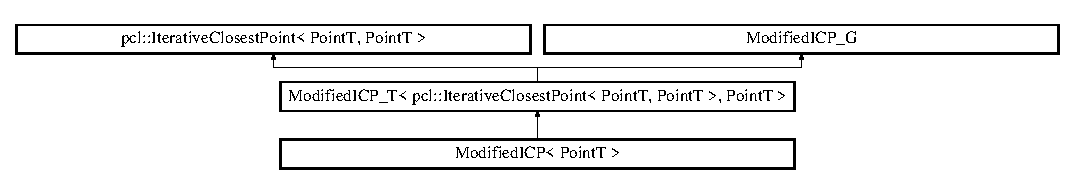
\includegraphics[height=2.043796cm]{classModifiedICP}
\end{center}
\end{figure}


\subsection{Detailed Description}
\subsubsection*{template$<$class PointT$>$ class ModifiedICP$<$ PointT $>$}

modified icp with icp 

The documentation for this class was generated from the following file:\begin{DoxyCompactItemize}
\item 
common/include/registration/impl/modified\_\-icp.hpp\end{DoxyCompactItemize}

\hypertarget{classModifiedICP__G}{
\section{ModifiedICP\_\-G Class Reference}
\label{classModifiedICP__G}\index{ModifiedICP\_\-G@{ModifiedICP\_\-G}}
}


{\ttfamily \#include $<$modified\_\-icp.hpp$>$}

Inheritance diagram for ModifiedICP\_\-G:\begin{figure}[H]
\begin{center}
\leavevmode
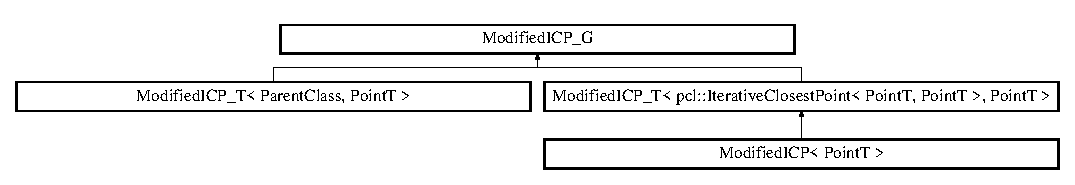
\includegraphics[height=2.043796cm]{classModifiedICP__G}
\end{center}
\end{figure}
\subsection*{Public Member Functions}
\begin{DoxyCompactItemize}
\item 
\hypertarget{classModifiedICP__G_ae519935eb1eb99432cef5f5b9d222758}{
virtual void {\bfseries setLM} ()=0}
\label{classModifiedICP__G_ae519935eb1eb99432cef5f5b9d222758}

\item 
\hypertarget{classModifiedICP__G_a02cec78304467b3babd3d096f634d722}{
virtual void {\bfseries setSearchFeatures} (\hyperlink{classFeatureContainerInterface}{FeatureContainerInterface} $\ast$features)=0}
\label{classModifiedICP__G_a02cec78304467b3babd3d096f634d722}

\end{DoxyCompactItemize}


\subsection{Detailed Description}
interface for setting up icp and derivats needed to use different backends 

The documentation for this class was generated from the following file:\begin{DoxyCompactItemize}
\item 
common/include/registration/impl/modified\_\-icp.hpp\end{DoxyCompactItemize}

\hypertarget{classModifiedICP__T}{
\section{ModifiedICP\_\-T$<$ ParentClass, PointT $>$ Class Template Reference}
\label{classModifiedICP__T}\index{ModifiedICP\_\-T@{ModifiedICP\_\-T}}
}


{\ttfamily \#include $<$modified\_\-icp.hpp$>$}

Inheritance diagram for ModifiedICP\_\-T$<$ ParentClass, PointT $>$:\begin{figure}[H]
\begin{center}
\leavevmode
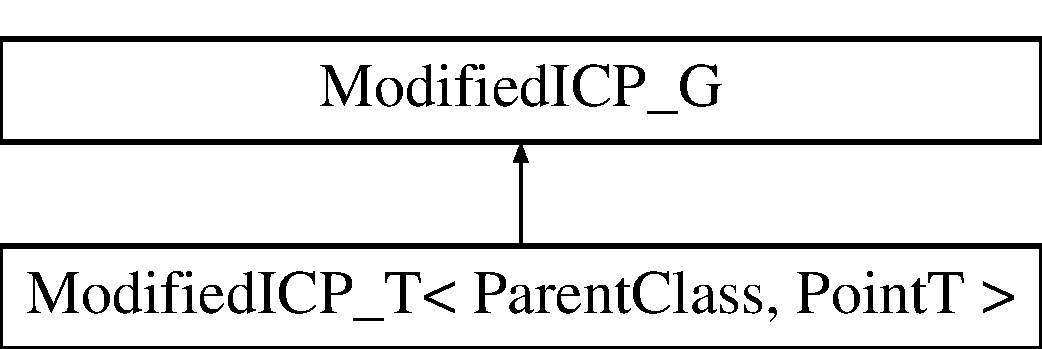
\includegraphics[height=2.000000cm]{classModifiedICP__T}
\end{center}
\end{figure}
\subsection*{Classes}
\begin{DoxyCompactItemize}
\item 
class {\bfseries FeatureSearch}
\end{DoxyCompactItemize}
\subsection*{Public Member Functions}
\begin{DoxyCompactItemize}
\item 
\hypertarget{classModifiedICP__T_a8010f52f6d5b496b33054094275110c2}{
int \hyperlink{classModifiedICP__T_a8010f52f6d5b496b33054094275110c2}{getNeededIterations} ()}
\label{classModifiedICP__T_a8010f52f6d5b496b33054094275110c2}

\begin{DoxyCompactList}\small\item\em get the needed iteration for computing \item\end{DoxyCompactList}\item 
\hypertarget{classModifiedICP__T_af010b080c2eb34971ecbdf2b2d356ad2}{
void \hyperlink{classModifiedICP__T_af010b080c2eb34971ecbdf2b2d356ad2}{setLM} ()}
\label{classModifiedICP__T_af010b080c2eb34971ecbdf2b2d356ad2}

\begin{DoxyCompactList}\small\item\em use LM instead of SVD (since pcl 1.3) \item\end{DoxyCompactList}\item 
\hypertarget{classModifiedICP__T_a508debe53bec7d8119cd26238d72b768}{
void \hyperlink{classModifiedICP__T_a508debe53bec7d8119cd26238d72b768}{setSearchFeatures} (\hyperlink{classFeatureContainerInterface}{FeatureContainerInterface} $\ast$features)}
\label{classModifiedICP__T_a508debe53bec7d8119cd26238d72b768}

\begin{DoxyCompactList}\small\item\em setup distance metric (hack for features) \item\end{DoxyCompactList}\end{DoxyCompactItemize}


\subsection{Detailed Description}
\subsubsection*{template$<$typename ParentClass, typename PointT$>$ class ModifiedICP\_\-T$<$ ParentClass, PointT $>$}

the modified icp allows (in pcl 1.1) to use own distance metric and obtaining the number of needed iterations 

The documentation for this class was generated from the following file:\begin{DoxyCompactItemize}
\item 
common/include/registration/impl/modified\_\-icp.hpp\end{DoxyCompactItemize}

\hypertarget{structNarfKPoint}{
\section{NarfKPoint Struct Reference}
\label{structNarfKPoint}\index{NarfKPoint@{NarfKPoint}}
}
\subsection*{Public Attributes}
\begin{DoxyCompactItemize}
\item 
\hypertarget{structNarfKPoint_ac9343633473e4f247b041b71c171442a}{
{\bfseries PCL\_\-ADD\_\-POINT4D}}
\label{structNarfKPoint_ac9343633473e4f247b041b71c171442a}

\item 
\hypertarget{structNarfKPoint_a6b489582876c17cad61805e8fa9caa9d}{
pcl::FPFHSignature33 {\bfseries fpfh}}
\label{structNarfKPoint_a6b489582876c17cad61805e8fa9caa9d}

\end{DoxyCompactItemize}


The documentation for this struct was generated from the following file:\begin{DoxyCompactItemize}
\item 
common/include/registration/features/narf\_\-kp.h\end{DoxyCompactItemize}

\hypertarget{classParameterBag}{
\section{ParameterBag Class Reference}
\label{classParameterBag}\index{ParameterBag@{ParameterBag}}
}
Inheritance diagram for ParameterBag:\begin{figure}[H]
\begin{center}
\leavevmode
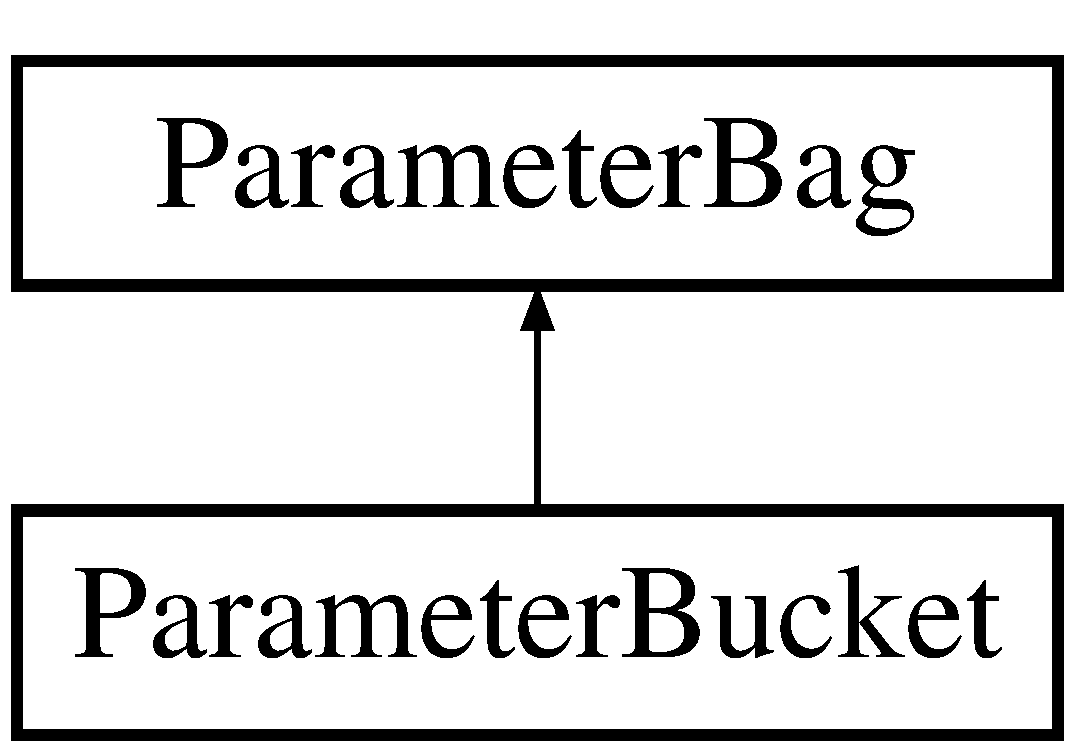
\includegraphics[height=2.000000cm]{classParameterBag}
\end{center}
\end{figure}
\subsection*{Classes}
\begin{DoxyCompactItemize}
\item 
struct \hyperlink{structParameterBag_1_1ParameterBagShortcut}{ParameterBagShortcut}
\end{DoxyCompactItemize}
\subsection*{Public Member Functions}
\begin{DoxyCompactItemize}
\item 
\hypertarget{classParameterBag_aa441186069d8890e7ecd94bc323b029d}{
const std::map$<$ std::string, int $>$ \& {\bfseries getInts} () const }
\label{classParameterBag_aa441186069d8890e7ecd94bc323b029d}

\item 
\hypertarget{classParameterBag_ab13e8fbb42358e4dc2f72456e0475ffa}{
const std::map$<$ std::string, double $>$ \& {\bfseries getDoubles} () const }
\label{classParameterBag_ab13e8fbb42358e4dc2f72456e0475ffa}

\item 
\hypertarget{classParameterBag_a96eab8894314fbced498b8a9025bdb59}{
const std::map$<$ std::string, std::string $>$ \& {\bfseries getStrings} () const }
\label{classParameterBag_a96eab8894314fbced498b8a9025bdb59}

\item 
\hypertarget{classParameterBag_ad3f0af8e03332d8ff072c2b087f447f0}{
\hyperlink{structParameterBag_1_1ParameterBagShortcut}{ParameterBagShortcut}$<$ int $>$ {\bfseries createParam} (ros::NodeHandle \&n, const std::string \&name, int v)}
\label{classParameterBag_ad3f0af8e03332d8ff072c2b087f447f0}

\item 
\hypertarget{classParameterBag_a6234beff97e34bae792f560dc5199700}{
\hyperlink{structParameterBag_1_1ParameterBagShortcut}{ParameterBagShortcut}$<$ double $>$ {\bfseries createParam} (ros::NodeHandle \&n, const std::string \&name, double v)}
\label{classParameterBag_a6234beff97e34bae792f560dc5199700}

\item 
\hypertarget{classParameterBag_aaf837b9c32c883471acd38825c8b415a}{
void {\bfseries createParam} (ros::NodeHandle \&n, const std::string \&name, std::string v)}
\label{classParameterBag_aaf837b9c32c883471acd38825c8b415a}

\item 
\hypertarget{classParameterBag_abd3c8663bf3b04bbb0f3978a87b31a2b}{
void {\bfseries setParam} (const std::string \&name, int v)}
\label{classParameterBag_abd3c8663bf3b04bbb0f3978a87b31a2b}

\item 
\hypertarget{classParameterBag_ab1157303d340f800f24245b1ec369b8b}{
void {\bfseries setParam} (const std::string \&name, const std::string \&v)}
\label{classParameterBag_ab1157303d340f800f24245b1ec369b8b}

\item 
\hypertarget{classParameterBag_ab862e0710eb048d59fff94cce04056af}{
void {\bfseries setParam} (const std::string \&name, double v)}
\label{classParameterBag_ab862e0710eb048d59fff94cce04056af}

\item 
\hypertarget{classParameterBag_a57d7a5cad5c90a8532cd93f61eefc37f}{
bool {\bfseries getParam} (const std::string \&name, int \&val)}
\label{classParameterBag_a57d7a5cad5c90a8532cd93f61eefc37f}

\item 
\hypertarget{classParameterBag_a8803c44d95e9341f3e9e746dcb71c06e}{
bool {\bfseries getParam} (const std::string \&name, double \&val)}
\label{classParameterBag_a8803c44d95e9341f3e9e746dcb71c06e}

\item 
\hypertarget{classParameterBag_a1b5b8dd08eef223b17333dbc982caea3}{
bool {\bfseries getParam} (const std::string \&name, std::string \&val)}
\label{classParameterBag_a1b5b8dd08eef223b17333dbc982caea3}

\item 
\hypertarget{classParameterBag_a2b0507694ac0f2606aec122621aa01ff}{
bool {\bfseries getMax} (const std::string \&name, int \&val)}
\label{classParameterBag_a2b0507694ac0f2606aec122621aa01ff}

\item 
\hypertarget{classParameterBag_a0db46a3c07d31177be78eba42f1b741d}{
bool {\bfseries getMax} (const std::string \&name, double \&val)}
\label{classParameterBag_a0db46a3c07d31177be78eba42f1b741d}

\item 
\hypertarget{classParameterBag_ab6521af4306ac281dfc92f9abc17f41d}{
bool {\bfseries getMin} (const std::string \&name, int \&val)}
\label{classParameterBag_ab6521af4306ac281dfc92f9abc17f41d}

\item 
\hypertarget{classParameterBag_ad25c1fae4a2049a1006d4b0c5eb13733}{
bool {\bfseries getMin} (const std::string \&name, double \&val)}
\label{classParameterBag_ad25c1fae4a2049a1006d4b0c5eb13733}

\item 
\hypertarget{classParameterBag_ad9c3ffc8b8cffe53196df06e34fdb1bf}{
bool {\bfseries getStep} (const std::string \&name, int \&val)}
\label{classParameterBag_ad9c3ffc8b8cffe53196df06e34fdb1bf}

\item 
\hypertarget{classParameterBag_aeb4a3e10ed52ff77d94d6a135a150be6}{
bool {\bfseries getStep} (const std::string \&name, double \&val)}
\label{classParameterBag_aeb4a3e10ed52ff77d94d6a135a150be6}

\end{DoxyCompactItemize}


The documentation for this class was generated from the following file:\begin{DoxyCompactItemize}
\item 
ros/src/parameters/parameters\_\-bag.h\end{DoxyCompactItemize}

\hypertarget{structParameterBag_1_1ParameterBagShortcut}{
\section{ParameterBag::ParameterBagShortcut$<$ T $>$ Struct Template Reference}
\label{structParameterBag_1_1ParameterBagShortcut}\index{ParameterBag::ParameterBagShortcut@{ParameterBag::ParameterBagShortcut}}
}
\subsection*{Public Member Functions}
\begin{DoxyCompactItemize}
\item 
\hypertarget{structParameterBag_1_1ParameterBagShortcut_a84ae8e98fbae020b1cacce1a8398d987}{
\hyperlink{structParameterBag_1_1ParameterBagShortcut}{ParameterBagShortcut} {\bfseries setMax} (T v)}
\label{structParameterBag_1_1ParameterBagShortcut_a84ae8e98fbae020b1cacce1a8398d987}

\item 
\hypertarget{structParameterBag_1_1ParameterBagShortcut_a0a99368a10b8bda439ea8c9f4699e47e}{
\hyperlink{structParameterBag_1_1ParameterBagShortcut}{ParameterBagShortcut} {\bfseries setMin} (T v)}
\label{structParameterBag_1_1ParameterBagShortcut_a0a99368a10b8bda439ea8c9f4699e47e}

\item 
\hypertarget{structParameterBag_1_1ParameterBagShortcut_aefc28bf99c830f7aa85ab1861ea793c2}{
\hyperlink{structParameterBag_1_1ParameterBagShortcut}{ParameterBagShortcut} {\bfseries setStep} (T v)}
\label{structParameterBag_1_1ParameterBagShortcut_aefc28bf99c830f7aa85ab1861ea793c2}

\end{DoxyCompactItemize}
\subsection*{Public Attributes}
\begin{DoxyCompactItemize}
\item 
\hypertarget{structParameterBag_1_1ParameterBagShortcut_add5034da70cd19af07c6cb8cd5a17154}{
std::string {\bfseries name}}
\label{structParameterBag_1_1ParameterBagShortcut_add5034da70cd19af07c6cb8cd5a17154}

\item 
\hypertarget{structParameterBag_1_1ParameterBagShortcut_a2b0c847a34ffd9140a3aa79ff2b21e39}{
\hyperlink{classParameterBag}{ParameterBag} $\ast$ {\bfseries p}}
\label{structParameterBag_1_1ParameterBagShortcut_a2b0c847a34ffd9140a3aa79ff2b21e39}

\end{DoxyCompactItemize}
\subsubsection*{template$<$typename T$>$ struct ParameterBag::ParameterBagShortcut$<$ T $>$}



The documentation for this struct was generated from the following file:\begin{DoxyCompactItemize}
\item 
ros/src/parameters/parameters\_\-bag.h\end{DoxyCompactItemize}

\hypertarget{classParameterBucket}{
\section{ParameterBucket Class Reference}
\label{classParameterBucket}\index{ParameterBucket@{ParameterBucket}}
}
Inheritance diagram for ParameterBucket:\begin{figure}[H]
\begin{center}
\leavevmode
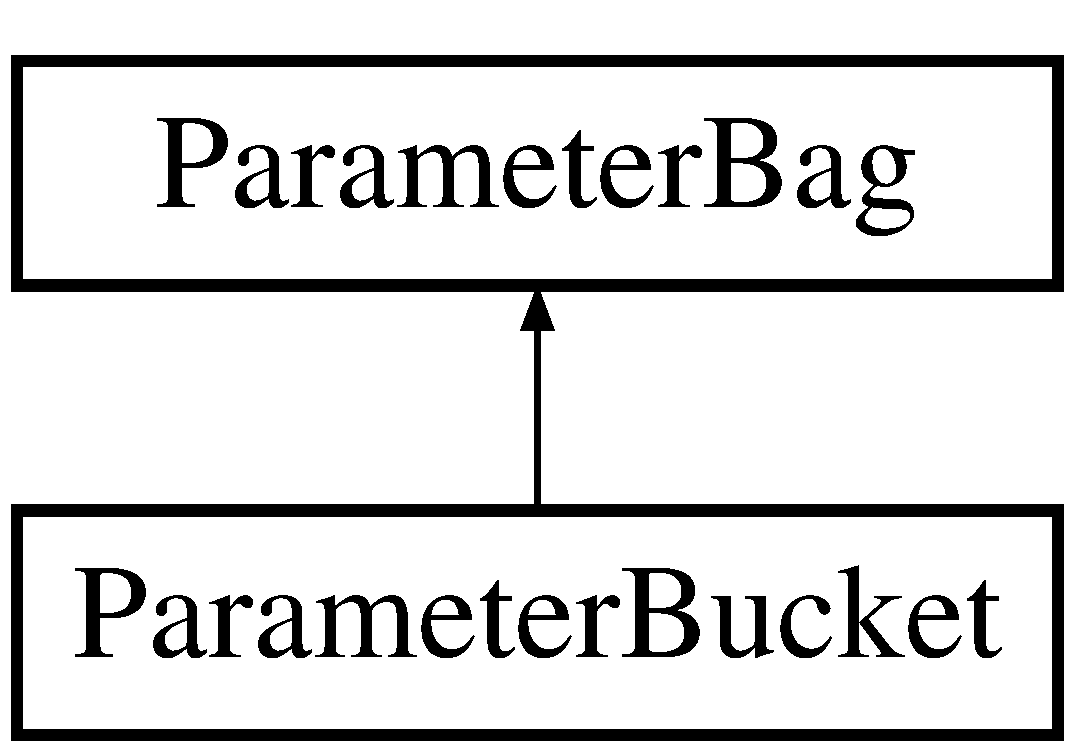
\includegraphics[height=2.000000cm]{classParameterBucket}
\end{center}
\end{figure}
\subsection*{Public Member Functions}
\begin{DoxyCompactItemize}
\item 
\hypertarget{classParameterBucket_a4e5220ad774903c93d62400508604d01}{
{\bfseries ParameterBucket} (ros::NodeHandle \&n)}
\label{classParameterBucket_a4e5220ad774903c93d62400508604d01}

\item 
\hypertarget{classParameterBucket_af2e5e3fd787b7f8962bdedd1dc1616a8}{
bool {\bfseries addParameter} (const std::string \&name)}
\label{classParameterBucket_af2e5e3fd787b7f8962bdedd1dc1616a8}

\end{DoxyCompactItemize}


The documentation for this class was generated from the following file:\begin{DoxyCompactItemize}
\item 
ros/src/parameters/parameters\_\-bag.h\end{DoxyCompactItemize}

\hypertarget{structPCAPoint}{
\section{PCAPoint Struct Reference}
\label{structPCAPoint}\index{PCAPoint@{PCAPoint}}
}
\subsection*{Public Attributes}
\begin{DoxyCompactItemize}
\item 
\hypertarget{structPCAPoint_aa9e39bf814ad72ad68072a09f4bc61e0}{
{\bfseries PCL\_\-ADD\_\-POINT4D}}
\label{structPCAPoint_aa9e39bf814ad72ad68072a09f4bc61e0}

\item 
\hypertarget{structPCAPoint_a5857d69a72eddbcae53c40f8ca8d1978}{
float {\bfseries data\_\-c} \mbox{[}9\mbox{]}}
\label{structPCAPoint_a5857d69a72eddbcae53c40f8ca8d1978}

\end{DoxyCompactItemize}


The documentation for this struct was generated from the following file:\begin{DoxyCompactItemize}
\item 
common/include/registration/features/segments.h\end{DoxyCompactItemize}

\hypertarget{classmeasurement__tools_1_1PrecisionStopWatchAll}{
\section{measurement\_\-tools::PrecisionStopWatchAll Class Reference}
\label{classmeasurement__tools_1_1PrecisionStopWatchAll}\index{measurement\_\-tools::PrecisionStopWatchAll@{measurement\_\-tools::PrecisionStopWatchAll}}
}


{\ttfamily \#include $<$time.h$>$}

\subsection*{Public Member Functions}
\begin{DoxyCompactItemize}
\item 
\hypertarget{classmeasurement__tools_1_1PrecisionStopWatchAll_adb5a8726007a23ba538e658c7f780ff6}{
void {\bfseries precisionStart} ()}
\label{classmeasurement__tools_1_1PrecisionStopWatchAll_adb5a8726007a23ba538e658c7f780ff6}

\item 
\hypertarget{classmeasurement__tools_1_1PrecisionStopWatchAll_aa413d864d8066718674424296ccb56ad}{
double {\bfseries precisionStop} ()}
\label{classmeasurement__tools_1_1PrecisionStopWatchAll_aa413d864d8066718674424296ccb56ad}

\end{DoxyCompactItemize}


\subsection{Detailed Description}
stop watch to measure duration 

The documentation for this class was generated from the following file:\begin{DoxyCompactItemize}
\item 
common/include/registration/measurements/time.h\end{DoxyCompactItemize}

\hypertarget{classmeasurement__tools_1_1PrecisionStopWatchThread}{
\section{measurement\_\-tools::PrecisionStopWatchThread Class Reference}
\label{classmeasurement__tools_1_1PrecisionStopWatchThread}\index{measurement\_\-tools::PrecisionStopWatchThread@{measurement\_\-tools::PrecisionStopWatchThread}}
}


{\ttfamily \#include $<$time.h$>$}

\subsection*{Public Member Functions}
\begin{DoxyCompactItemize}
\item 
\hypertarget{classmeasurement__tools_1_1PrecisionStopWatchThread_a0269d78125a6eb7f73942c8b391344c6}{
void {\bfseries precisionStart} ()}
\label{classmeasurement__tools_1_1PrecisionStopWatchThread_a0269d78125a6eb7f73942c8b391344c6}

\item 
\hypertarget{classmeasurement__tools_1_1PrecisionStopWatchThread_ad2f9a8faf4bb83a64535ebce7c8dad6e}{
double {\bfseries precisionStop} ()}
\label{classmeasurement__tools_1_1PrecisionStopWatchThread_ad2f9a8faf4bb83a64535ebce7c8dad6e}

\end{DoxyCompactItemize}


\subsection{Detailed Description}
stop watch to measure time needed by this thread 

The documentation for this class was generated from the following file:\begin{DoxyCompactItemize}
\item 
common/include/registration/measurements/time.h\end{DoxyCompactItemize}

\hypertarget{classRegistration__Corrospondence}{
\section{Registration\_\-Corrospondence$<$ Point $>$ Class Template Reference}
\label{classRegistration__Corrospondence}\index{Registration\_\-Corrospondence@{Registration\_\-Corrospondence}}
}
Inheritance diagram for Registration\_\-Corrospondence$<$ Point $>$:\begin{figure}[H]
\begin{center}
\leavevmode
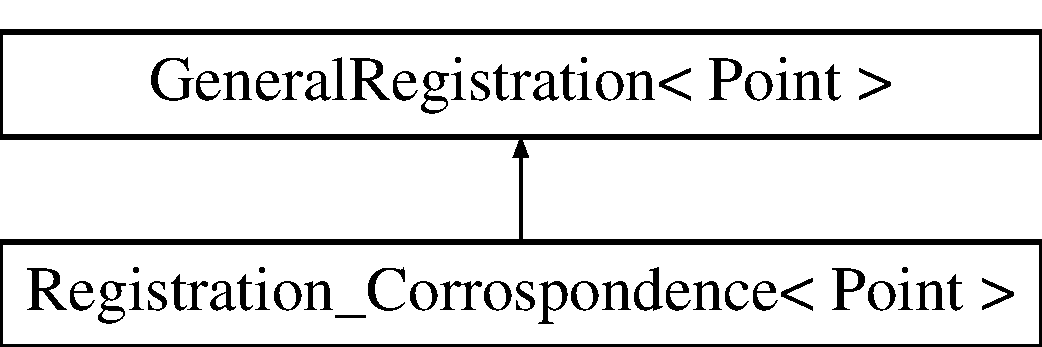
\includegraphics[height=2.000000cm]{classRegistration__Corrospondence}
\end{center}
\end{figure}
\subsection*{Public Member Functions}
\begin{DoxyCompactItemize}
\item 
\hypertarget{classRegistration__Corrospondence_ac23793781bc288e7d3255fe3fad21d95}{
void {\bfseries setKeypoints} (\hyperlink{classRegKeypointCorrespondenceAbstract}{RegKeypointCorrespondenceAbstract}$<$ Point $>$ $\ast$k)}
\label{classRegistration__Corrospondence_ac23793781bc288e7d3255fe3fad21d95}

\item 
\hypertarget{classRegistration__Corrospondence_aae93bc641218d3ffa81985b60a995c8b}{
\hyperlink{classRegKeypointCorrespondenceAbstract}{RegKeypointCorrespondenceAbstract}$<$ Point $>$ $\ast$ {\bfseries getKeypoints} ()}
\label{classRegistration__Corrospondence_aae93bc641218d3ffa81985b60a995c8b}

\end{DoxyCompactItemize}
\subsection*{Protected Member Functions}
\begin{DoxyCompactItemize}
\item 
\hypertarget{classRegistration__Corrospondence_ab1c6a8ed9e5348a145f2b434252b2539}{
virtual bool {\bfseries compute\_\-features} ()}
\label{classRegistration__Corrospondence_ab1c6a8ed9e5348a145f2b434252b2539}

\item 
\hypertarget{classRegistration__Corrospondence_a9a23608e726d2684f1e8f5813640bf19}{
virtual bool {\bfseries compute\_\-corrospondences} ()}
\label{classRegistration__Corrospondence_a9a23608e726d2684f1e8f5813640bf19}

\item 
\hypertarget{classRegistration__Corrospondence_ac7c2a2308d4927d5811077e91c253818}{
virtual bool {\bfseries compute\_\-transformation} ()}
\label{classRegistration__Corrospondence_ac7c2a2308d4927d5811077e91c253818}

\item 
\hypertarget{classRegistration__Corrospondence_a3dcc8134ad1f7c80ab135e5babff4ca8}{
void {\bfseries rejectBadCorrespondences} (const pcl::registration::CorrespondencesPtr \&all\_\-correspondences, pcl::registration::Correspondences \&remaining\_\-correspondences)}
\label{classRegistration__Corrospondence_a3dcc8134ad1f7c80ab135e5babff4ca8}

\end{DoxyCompactItemize}
\subsection*{Protected Attributes}
\begin{DoxyCompactItemize}
\item 
\hypertarget{classRegistration__Corrospondence_a930bedcad3a53b8616b15a0bb8b4afd1}{
pcl::PointCloud$<$ Point $>$ {\bfseries register\_\-}}
\label{classRegistration__Corrospondence_a930bedcad3a53b8616b15a0bb8b4afd1}

\item 
\hypertarget{classRegistration__Corrospondence_ab024cf1136295f16c4786c874b91e436}{
float {\bfseries rejection\_\-dis\_\-}}
\label{classRegistration__Corrospondence_ab024cf1136295f16c4786c874b91e436}

\item 
\hypertarget{classRegistration__Corrospondence_a10bf2e0005a1a7dbaa4daf43b1f8c8bf}{
\hyperlink{classRegKeypointCorrespondenceAbstract}{RegKeypointCorrespondenceAbstract}$<$ Point $>$ $\ast$ {\bfseries keypoints\_\-}}
\label{classRegistration__Corrospondence_a10bf2e0005a1a7dbaa4daf43b1f8c8bf}

\item 
\hypertarget{classRegistration__Corrospondence_a657b233d8150bf90131727f583f20c6f}{
pcl::registration::CorrespondencesPtr {\bfseries all\_\-correspondences\_\-}}
\label{classRegistration__Corrospondence_a657b233d8150bf90131727f583f20c6f}

\end{DoxyCompactItemize}
\subsubsection*{template$<$typename Point$>$ class Registration\_\-Corrospondence$<$ Point $>$}



The documentation for this class was generated from the following files:\begin{DoxyCompactItemize}
\item 
common/include/registration/registration\_\-correspondence.h\item 
common/include/registration/impl/registration\_\-correspondence.hpp\end{DoxyCompactItemize}

\hypertarget{classRegistration__FastSLAM}{
\section{Registration\_\-FastSLAM$<$ Point $>$ Class Template Reference}
\label{classRegistration__FastSLAM}\index{Registration\_\-FastSLAM@{Registration\_\-FastSLAM}}
}
Inheritance diagram for Registration\_\-FastSLAM$<$ Point $>$:\begin{figure}[H]
\begin{center}
\leavevmode
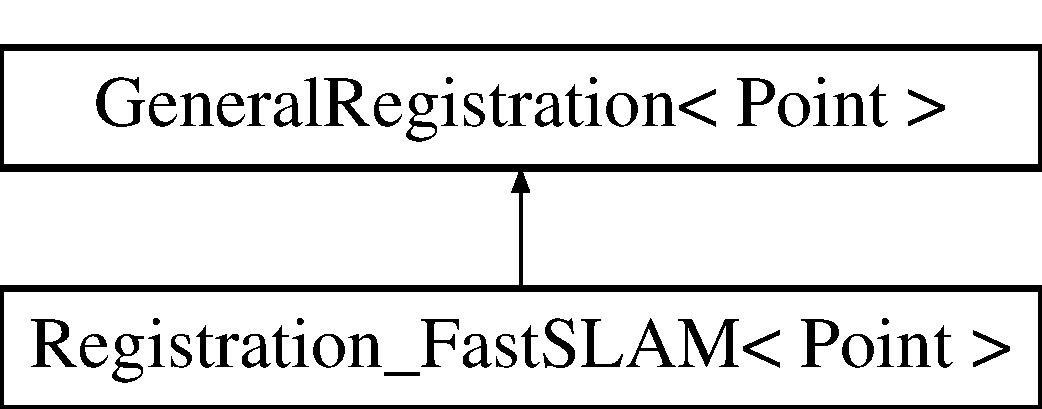
\includegraphics[height=2.000000cm]{classRegistration__FastSLAM}
\end{center}
\end{figure}
\subsection*{Public Member Functions}
\begin{DoxyCompactItemize}
\item 
\hypertarget{classRegistration__FastSLAM_ae7ed9dcde8de4c5b5669e407db039049}{
virtual boost::shared\_\-ptr$<$ const pcl::PointCloud$<$ Point $>$ $>$ \hyperlink{classRegistration__FastSLAM_ae7ed9dcde8de4c5b5669e407db039049}{getMarkers} ()}
\label{classRegistration__FastSLAM_ae7ed9dcde8de4c5b5669e407db039049}

\begin{DoxyCompactList}\small\item\em debug function for marker visualization \item\end{DoxyCompactList}\end{DoxyCompactItemize}
\subsection*{Protected Member Functions}
\begin{DoxyCompactItemize}
\item 
\hypertarget{classRegistration__FastSLAM_a69665dced66ca9652faa3df9dfc9c7c8}{
virtual bool {\bfseries compute\_\-features} ()}
\label{classRegistration__FastSLAM_a69665dced66ca9652faa3df9dfc9c7c8}

\item 
virtual bool \hyperlink{classRegistration__FastSLAM_a2f82b64987bd1aa8393c5b45f31fc13d}{compute\_\-corrospondences} ()
\item 
\hypertarget{classRegistration__FastSLAM_ac887352313d157d292fd39b20893a350}{
virtual bool {\bfseries compute\_\-transformation} ()}
\label{classRegistration__FastSLAM_ac887352313d157d292fd39b20893a350}

\item 
\hypertarget{classRegistration__FastSLAM_ab282d236ae291f06d9a7d707f840a12e}{
virtual boost::shared\_\-ptr$<$ pcl::PointCloud$<$ Point $>$ $>$ \hyperlink{classRegistration__FastSLAM_ab282d236ae291f06d9a7d707f840a12e}{getMap} ()}
\label{classRegistration__FastSLAM_ab282d236ae291f06d9a7d707f840a12e}

\begin{DoxyCompactList}\small\item\em map is not necessarily implemented \item\end{DoxyCompactList}\end{DoxyCompactItemize}
\subsubsection*{template$<$typename Point$>$ class Registration\_\-FastSLAM$<$ Point $>$}



\subsection{Member Function Documentation}
\hypertarget{classRegistration__FastSLAM_a2f82b64987bd1aa8393c5b45f31fc13d}{
\index{Registration\_\-FastSLAM@{Registration\_\-FastSLAM}!compute\_\-corrospondences@{compute\_\-corrospondences}}
\index{compute\_\-corrospondences@{compute\_\-corrospondences}!Registration_FastSLAM@{Registration\_\-FastSLAM}}
\subsubsection[{compute\_\-corrospondences}]{\setlength{\rightskip}{0pt plus 5cm}template$<$typename Point $>$ virtual bool {\bf Registration\_\-FastSLAM}$<$ Point $>$::compute\_\-corrospondences (
\begin{DoxyParamCaption}
{}
\end{DoxyParamCaption}
)\hspace{0.3cm}{\ttfamily  \mbox{[}inline, protected, virtual\mbox{]}}}}
\label{classRegistration__FastSLAM_a2f82b64987bd1aa8393c5b45f31fc13d}


Remove class associations from rejected particles

Remove class label if necessary

Add new feature only if it is not masked It is important that the features ID corresponds to the position in the particle map 



Implements \hyperlink{classGeneralRegistration}{GeneralRegistration$<$ Point $>$}.



The documentation for this class was generated from the following file:\begin{DoxyCompactItemize}
\item 
common/include/registration/registration\_\-fastslam.h\end{DoxyCompactItemize}

\hypertarget{classRegistration__ICP}{
\section{Registration\_\-ICP$<$ Point $>$ Class Template Reference}
\label{classRegistration__ICP}\index{Registration\_\-ICP@{Registration\_\-ICP}}
}


{\ttfamily \#include $<$registration\_\-icp.h$>$}

Inheritance diagram for Registration\_\-ICP$<$ Point $>$:\begin{figure}[H]
\begin{center}
\leavevmode
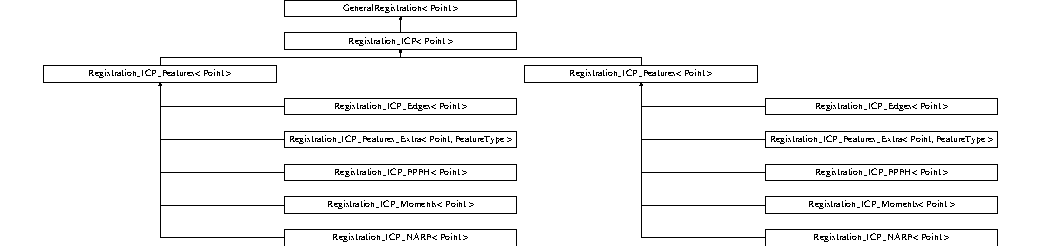
\includegraphics[height=3.303835cm]{classRegistration__ICP}
\end{center}
\end{figure}
\subsection*{Public Member Functions}
\begin{DoxyCompactItemize}
\item 
\hypertarget{classRegistration__ICP_ab16c8d926cbfaefec2cfb5e29eceffab}{
void \hyperlink{classRegistration__ICP_ab16c8d926cbfaefec2cfb5e29eceffab}{setNonLinear} (bool b)}
\label{classRegistration__ICP_ab16c8d926cbfaefec2cfb5e29eceffab}

\begin{DoxyCompactList}\small\item\em non linear uses LM instead of SVD \item\end{DoxyCompactList}\item 
\hypertarget{classRegistration__ICP_a248f3d67674df34036faaccf7f69f014}{
void \hyperlink{classRegistration__ICP_a248f3d67674df34036faaccf7f69f014}{setUseOnlyLastReference} (bool b)}
\label{classRegistration__ICP_a248f3d67674df34036faaccf7f69f014}

\begin{DoxyCompactList}\small\item\em set false to build up a map, instead of using only last frame for registration \item\end{DoxyCompactList}\item 
\hypertarget{classRegistration__ICP_ae577aec867b0d2f350487dceba478b64}{
void \hyperlink{classRegistration__ICP_ae577aec867b0d2f350487dceba478b64}{setUseGICP} (bool b)}
\label{classRegistration__ICP_ae577aec867b0d2f350487dceba478b64}

\begin{DoxyCompactList}\small\item\em switch backend to gicp \item\end{DoxyCompactList}\item 
\hypertarget{classRegistration__ICP_a5eb9c15e9b4cf56f676a7e73d0855b82}{
virtual boost::shared\_\-ptr$<$ pcl::PointCloud$<$ Point $>$ $>$ \hyperlink{classRegistration__ICP_a5eb9c15e9b4cf56f676a7e73d0855b82}{getMap} ()}
\label{classRegistration__ICP_a5eb9c15e9b4cf56f676a7e73d0855b82}

\begin{DoxyCompactList}\small\item\em return pointlcoud to register against \item\end{DoxyCompactList}\item 
\hypertarget{classRegistration__ICP_a00182a197453a61cdd58108e0cd9fb6f}{
void \hyperlink{classRegistration__ICP_a00182a197453a61cdd58108e0cd9fb6f}{setMaxIterations} (int v)}
\label{classRegistration__ICP_a00182a197453a61cdd58108e0cd9fb6f}

\begin{DoxyCompactList}\small\item\em set maximum number of iterations \item\end{DoxyCompactList}\item 
\hypertarget{classRegistration__ICP_a24520c9711a60d047c107664426e7d33}{
void \hyperlink{classRegistration__ICP_a24520c9711a60d047c107664426e7d33}{setCorrDist} (float v)}
\label{classRegistration__ICP_a24520c9711a60d047c107664426e7d33}

\begin{DoxyCompactList}\small\item\em set maximum correlation distance \item\end{DoxyCompactList}\item 
\hypertarget{classRegistration__ICP_aa13488b9d37d5edf16baaf3de11242ba}{
void \hyperlink{classRegistration__ICP_aa13488b9d37d5edf16baaf3de11242ba}{setTrfEpsilon} (float v)}
\label{classRegistration__ICP_aa13488b9d37d5edf16baaf3de11242ba}

\begin{DoxyCompactList}\small\item\em sets transformation epsilon as break condition for icp \item\end{DoxyCompactList}\item 
\hypertarget{classRegistration__ICP_a648647c59a5693170332c17e328dec39}{
void \hyperlink{classRegistration__ICP_a648647c59a5693170332c17e328dec39}{setOutlierRejectionThreshold} (float v)}
\label{classRegistration__ICP_a648647c59a5693170332c17e328dec39}

\begin{DoxyCompactList}\small\item\em sets maximum distance for RANSAC \item\end{DoxyCompactList}\end{DoxyCompactItemize}
\subsection*{Protected Member Functions}
\begin{DoxyCompactItemize}
\item 
\hypertarget{classRegistration__ICP_a656bded6e531c0ed9e23a0851d0c97dc}{
virtual bool {\bfseries compute\_\-features} ()}
\label{classRegistration__ICP_a656bded6e531c0ed9e23a0851d0c97dc}

\item 
\hypertarget{classRegistration__ICP_aa375b4ac4304c0055fa15452046f77a3}{
virtual bool {\bfseries compute\_\-corrospondences} ()}
\label{classRegistration__ICP_aa375b4ac4304c0055fa15452046f77a3}

\item 
\hypertarget{classRegistration__ICP_ad016a9ee4ae532da959c397e6990d2fd}{
virtual bool {\bfseries compute\_\-transformation} ()}
\label{classRegistration__ICP_ad016a9ee4ae532da959c397e6990d2fd}

\item 
virtual void \hyperlink{classRegistration__ICP_a3217a0d69daa6726a5c8049600b9607a}{setSettingsForICP} (\hyperlink{classModifiedICP__G}{ModifiedICP\_\-G} $\ast$icp)
\end{DoxyCompactItemize}
\subsection*{Protected Attributes}
\begin{DoxyCompactItemize}
\item 
\hypertarget{classRegistration__ICP_a20abdf17fe5018793562e5ee6846d21f}{
pcl::PointCloud$<$ Point $>$ {\bfseries register\_\-}}
\label{classRegistration__ICP_a20abdf17fe5018793562e5ee6846d21f}

\item 
\hypertarget{classRegistration__ICP_a5e42b414fed6c9819ee9f32c823ec1ae}{
int {\bfseries icp\_\-max\_\-iterations\_\-}}
\label{classRegistration__ICP_a5e42b414fed6c9819ee9f32c823ec1ae}

\item 
\hypertarget{classRegistration__ICP_aca82c8a16a506d961391953d066a2fe4}{
float {\bfseries icp\_\-max\_\-corr\_\-dist\_\-}}
\label{classRegistration__ICP_aca82c8a16a506d961391953d066a2fe4}

\item 
\hypertarget{classRegistration__ICP_a8f16700511ebd07a622729917f12d8c9}{
float {\bfseries outlier\_\-rejection\_\-threshold\_\-}}
\label{classRegistration__ICP_a8f16700511ebd07a622729917f12d8c9}

\item 
\hypertarget{classRegistration__ICP_ad7e975482bc81a2c49fa82b7d29758d8}{
float {\bfseries icp\_\-trf\_\-epsilon\_\-}}
\label{classRegistration__ICP_ad7e975482bc81a2c49fa82b7d29758d8}

\item 
\hypertarget{classRegistration__ICP_a09bf9b060c676380761a75cc7831f642}{
bool {\bfseries non\_\-linear\_\-}}
\label{classRegistration__ICP_a09bf9b060c676380761a75cc7831f642}

\item 
\hypertarget{classRegistration__ICP_af46d619b7417a00a925b3557ea3e771d}{
bool {\bfseries use\_\-only\_\-last\_\-refrence\_\-}}
\label{classRegistration__ICP_af46d619b7417a00a925b3557ea3e771d}

\item 
\hypertarget{classRegistration__ICP_ab471192a1045e731608aead65acdffad}{
bool {\bfseries use\_\-gicp\_\-}}
\label{classRegistration__ICP_ab471192a1045e731608aead65acdffad}

\end{DoxyCompactItemize}


\subsection{Detailed Description}
\subsubsection*{template$<$typename Point$>$ class Registration\_\-ICP$<$ Point $>$}

encapsulates icp with extension extending icp to allow featurebased matching, as keypoint matching 

\subsection{Member Function Documentation}
\hypertarget{classRegistration__ICP_a3217a0d69daa6726a5c8049600b9607a}{
\index{Registration\_\-ICP@{Registration\_\-ICP}!setSettingsForICP@{setSettingsForICP}}
\index{setSettingsForICP@{setSettingsForICP}!Registration_ICP@{Registration\_\-ICP}}
\subsubsection[{setSettingsForICP}]{\setlength{\rightskip}{0pt plus 5cm}template$<$typename Point $>$ void {\bf Registration\_\-ICP}$<$ Point $>$::setSettingsForICP (
\begin{DoxyParamCaption}
\item[{{\bf ModifiedICP\_\-G} $\ast$}]{ icp}
\end{DoxyParamCaption}
)\hspace{0.3cm}{\ttfamily  \mbox{[}protected, virtual\mbox{]}}}}
\label{classRegistration__ICP_a3217a0d69daa6726a5c8049600b9607a}
function for setting up icp can be overwritten by subclasses to modify backend 

Reimplemented in \hyperlink{classRegistration__ICP__Features_a944cd0d0d248afc66b9833f0cfd322ed}{Registration\_\-ICP\_\-Features$<$ Point $>$}.



The documentation for this class was generated from the following files:\begin{DoxyCompactItemize}
\item 
common/include/registration/registration\_\-icp.h\item 
common/include/registration/impl/registration\_\-icp.hpp\end{DoxyCompactItemize}

\hypertarget{classRegistration__ICP__Edges}{
\section{Registration\_\-ICP\_\-Edges$<$ Point $>$ Class Template Reference}
\label{classRegistration__ICP__Edges}\index{Registration\_\-ICP\_\-Edges@{Registration\_\-ICP\_\-Edges}}
}
Inheritance diagram for Registration\_\-ICP\_\-Edges$<$ Point $>$:\begin{figure}[H]
\begin{center}
\leavevmode
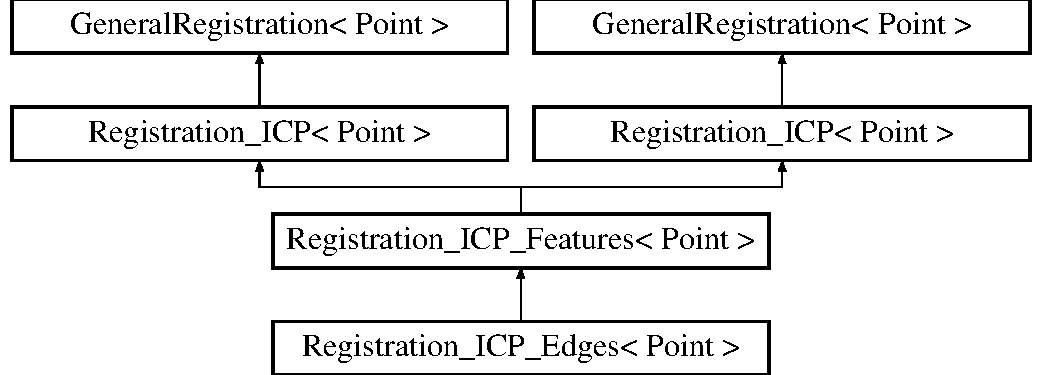
\includegraphics[height=4.000000cm]{classRegistration__ICP__Edges}
\end{center}
\end{figure}
\subsection*{Public Member Functions}
\begin{DoxyCompactItemize}
\item 
\hypertarget{classRegistration__ICP__Edges_a8b3d6bbb4e57f46c90c296545dcc51d0}{
virtual boost::shared\_\-ptr$<$ const pcl::PointCloud$<$ Point $>$ $>$ \hyperlink{classRegistration__ICP__Edges_a8b3d6bbb4e57f46c90c296545dcc51d0}{getMarkers} ()}
\label{classRegistration__ICP__Edges_a8b3d6bbb4e57f46c90c296545dcc51d0}

\begin{DoxyCompactList}\small\item\em debug function for marker visualization \item\end{DoxyCompactList}\item 
\hypertarget{classRegistration__ICP__Edges_a36d5d5fe3955b11e81610496147e2159}{
void {\bfseries setRadius} (float v)}
\label{classRegistration__ICP__Edges_a36d5d5fe3955b11e81610496147e2159}

\item 
\hypertarget{classRegistration__ICP__Edges_a4d108ccdabc085bf79d45ac9659d84e1}{
void {\bfseries setThreshold} (float v)}
\label{classRegistration__ICP__Edges_a4d108ccdabc085bf79d45ac9659d84e1}

\item 
\hypertarget{classRegistration__ICP__Edges_aad7c241aec15cb5f7543673ca47db8ea}{
void {\bfseries setDisThreshold} (float v)}
\label{classRegistration__ICP__Edges_aad7c241aec15cb5f7543673ca47db8ea}

\end{DoxyCompactItemize}
\subsection*{Protected Member Functions}
\begin{DoxyCompactItemize}
\item 
\hypertarget{classRegistration__ICP__Edges_aa83ea33070108e6b9d78efaeb86e772c}{
virtual bool {\bfseries compute\_\-features} ()}
\label{classRegistration__ICP__Edges_aa83ea33070108e6b9d78efaeb86e772c}

\item 
\hypertarget{classRegistration__ICP__Edges_adab7fe49642c35cc9ebe416ab2e7cd63}{
virtual bool {\bfseries compute\_\-transformation} ()}
\label{classRegistration__ICP__Edges_adab7fe49642c35cc9ebe416ab2e7cd63}

\end{DoxyCompactItemize}
\subsubsection*{template$<$typename Point$>$ class Registration\_\-ICP\_\-Edges$<$ Point $>$}



The documentation for this class was generated from the following file:\begin{DoxyCompactItemize}
\item 
common/include/registration/registration\_\-icp\_\-edges.h\end{DoxyCompactItemize}

\hypertarget{classRegistration__ICP__Features}{
\section{Registration\_\-ICP\_\-Features$<$ Point $>$ Class Template Reference}
\label{classRegistration__ICP__Features}\index{Registration\_\-ICP\_\-Features@{Registration\_\-ICP\_\-Features}}
}


{\ttfamily \#include $<$registration\_\-icp.h$>$}

Inheritance diagram for Registration\_\-ICP\_\-Features$<$ Point $>$:\begin{figure}[H]
\begin{center}
\leavevmode
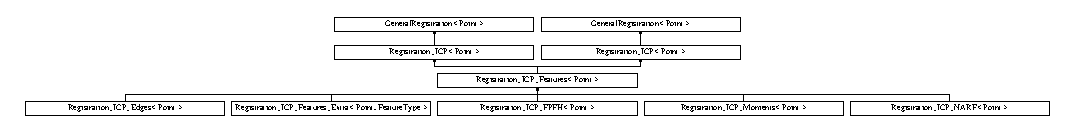
\includegraphics[height=1.321534cm]{classRegistration__ICP__Features}
\end{center}
\end{figure}
\subsection*{Public Member Functions}
\begin{DoxyCompactItemize}
\item 
void \hyperlink{classRegistration__ICP__Features_a63a46214a8b176447ba6ee0986d2dea5}{setFeatures} (\hyperlink{classFeatureContainerInterface}{FeatureContainerInterface} $\ast$features)
\end{DoxyCompactItemize}
\subsection*{Protected Member Functions}
\begin{DoxyCompactItemize}
\item 
virtual void \hyperlink{classRegistration__ICP__Features_a944cd0d0d248afc66b9833f0cfd322ed}{setSettingsForICP} (\hyperlink{classModifiedICP__G}{ModifiedICP\_\-G} $\ast$icp)
\item 
\hypertarget{classRegistration__ICP__Features_abbc0a01f50b62453b469a7f044751644}{
virtual void {\bfseries setSettingsForICP} (\hyperlink{classModifiedICP}{ModifiedICP}$<$ Point $>$ \&icp)}
\label{classRegistration__ICP__Features_abbc0a01f50b62453b469a7f044751644}

\end{DoxyCompactItemize}
\subsection*{Protected Attributes}
\begin{DoxyCompactItemize}
\item 
\hypertarget{classRegistration__ICP__Features_a1a47588deb521b8eaf140f262ab7511e}{
\hyperlink{classFeatureContainerInterface}{FeatureContainerInterface} $\ast$ {\bfseries features\_\-}}
\label{classRegistration__ICP__Features_a1a47588deb521b8eaf140f262ab7511e}

\item 
\hypertarget{classRegistration__ICP__Features_a8b93595575938bd37e96dd4bbdf5f8a7}{
const \hyperlink{classFeatureContainerInterface}{FeatureContainerInterface} $\ast$ {\bfseries features\_\-}}
\label{classRegistration__ICP__Features_a8b93595575938bd37e96dd4bbdf5f8a7}

\end{DoxyCompactItemize}


\subsection{Detailed Description}
\subsubsection*{template$<$typename Point$>$ class Registration\_\-ICP\_\-Features$<$ Point $>$}

extending icp to features and keypoints 

\subsection{Member Function Documentation}
\hypertarget{classRegistration__ICP__Features_a63a46214a8b176447ba6ee0986d2dea5}{
\index{Registration\_\-ICP\_\-Features@{Registration\_\-ICP\_\-Features}!setFeatures@{setFeatures}}
\index{setFeatures@{setFeatures}!Registration_ICP_Features@{Registration\_\-ICP\_\-Features}}
\subsubsection[{setFeatures}]{\setlength{\rightskip}{0pt plus 5cm}template$<$typename Point $>$ void {\bf Registration\_\-ICP\_\-Features}$<$ Point $>$::setFeatures (
\begin{DoxyParamCaption}
\item[{{\bf FeatureContainerInterface} $\ast$}]{ features}
\end{DoxyParamCaption}
)\hspace{0.3cm}{\ttfamily  \mbox{[}inline\mbox{]}}}}
\label{classRegistration__ICP__Features_a63a46214a8b176447ba6ee0986d2dea5}
sets a featureinterface it is used for the correlation calculation in icp \hypertarget{classRegistration__ICP__Features_a944cd0d0d248afc66b9833f0cfd322ed}{
\index{Registration\_\-ICP\_\-Features@{Registration\_\-ICP\_\-Features}!setSettingsForICP@{setSettingsForICP}}
\index{setSettingsForICP@{setSettingsForICP}!Registration_ICP_Features@{Registration\_\-ICP\_\-Features}}
\subsubsection[{setSettingsForICP}]{\setlength{\rightskip}{0pt plus 5cm}template$<$typename Point $>$ void {\bf Registration\_\-ICP\_\-Features}$<$ Point $>$::setSettingsForICP (
\begin{DoxyParamCaption}
\item[{{\bf ModifiedICP\_\-G} $\ast$}]{ icp}
\end{DoxyParamCaption}
)\hspace{0.3cm}{\ttfamily  \mbox{[}protected, virtual\mbox{]}}}}
\label{classRegistration__ICP__Features_a944cd0d0d248afc66b9833f0cfd322ed}
function for setting up icp can be overwritten by subclasses to modify backend 

Reimplemented from \hyperlink{classRegistration__ICP_a3217a0d69daa6726a5c8049600b9607a}{Registration\_\-ICP$<$ Point $>$}.



The documentation for this class was generated from the following files:\begin{DoxyCompactItemize}
\item 
common/include/registration/registration\_\-icp.h\item 
common/include/registration/registration\_\-moments.h\item 
common/include/registration/impl/registration\_\-icp.hpp\end{DoxyCompactItemize}

\hypertarget{classRegistration__ICP__Features__Extra}{
\section{Registration\_\-ICP\_\-Features\_\-Extra$<$ Point, FeatureType $>$ Class Template Reference}
\label{classRegistration__ICP__Features__Extra}\index{Registration\_\-ICP\_\-Features\_\-Extra@{Registration\_\-ICP\_\-Features\_\-Extra}}
}
Inheritance diagram for Registration\_\-ICP\_\-Features\_\-Extra$<$ Point, FeatureType $>$:\begin{figure}[H]
\begin{center}
\leavevmode
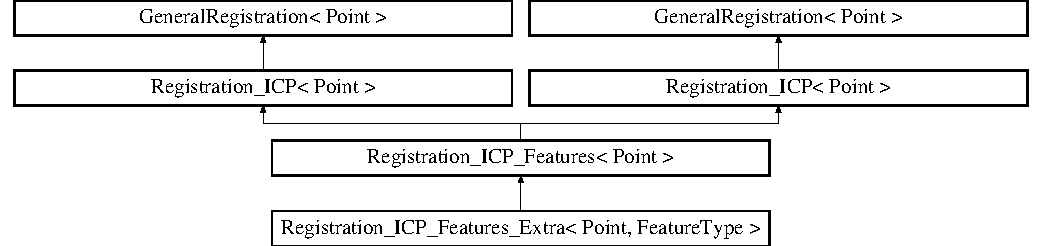
\includegraphics[height=3.303835cm]{classRegistration__ICP__Features__Extra}
\end{center}
\end{figure}
\subsection*{Public Member Functions}
\begin{DoxyCompactItemize}
\item 
\hypertarget{classRegistration__ICP__Features__Extra_a23c8c445eb40c1a84f3d725783ed43c3}{
virtual bool {\bfseries calculateFeature} (boost::shared\_\-ptr$<$ pcl::PointCloud$<$ Point $>$ $>$ input, boost::shared\_\-ptr$<$ pcl::PointCloud$<$ Point $>$ $>$ output, boost::shared\_\-ptr$<$ pcl::PointCloud$<$ FeatureType $>$ $>$ features)}
\label{classRegistration__ICP__Features__Extra_a23c8c445eb40c1a84f3d725783ed43c3}

\end{DoxyCompactItemize}
\subsection*{Protected Member Functions}
\begin{DoxyCompactItemize}
\item 
\hypertarget{classRegistration__ICP__Features__Extra_a16c5ac8403f6786f449e44b75684ab36}{
virtual bool {\bfseries compute\_\-features} ()}
\label{classRegistration__ICP__Features__Extra_a16c5ac8403f6786f449e44b75684ab36}

\end{DoxyCompactItemize}
\subsubsection*{template$<$typename Point, typename FeatureType$>$ class Registration\_\-ICP\_\-Features\_\-Extra$<$ Point, FeatureType $>$}



The documentation for this class was generated from the following files:\begin{DoxyCompactItemize}
\item 
common/include/registration/registration\_\-icp.h\item 
common/include/registration/impl/registration\_\-icp.hpp\end{DoxyCompactItemize}

\hypertarget{classRegistration__ICP__FPFH}{
\section{Registration\_\-ICP\_\-FPFH$<$ Point $>$ Class Template Reference}
\label{classRegistration__ICP__FPFH}\index{Registration\_\-ICP\_\-FPFH@{Registration\_\-ICP\_\-FPFH}}
}
Inheritance diagram for Registration\_\-ICP\_\-FPFH$<$ Point $>$:\begin{figure}[H]
\begin{center}
\leavevmode
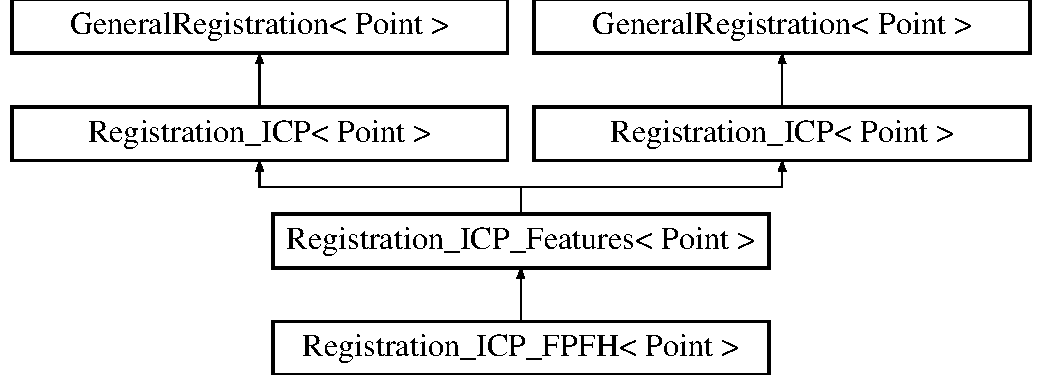
\includegraphics[height=4.000000cm]{classRegistration__ICP__FPFH}
\end{center}
\end{figure}
\subsection*{Public Member Functions}
\begin{DoxyCompactItemize}
\item 
\hypertarget{classRegistration__ICP__FPFH_ac6120c9fc679004668f6e4b16e31ac2b}{
void {\bfseries setFPFHRadius} (float v)}
\label{classRegistration__ICP__FPFH_ac6120c9fc679004668f6e4b16e31ac2b}

\end{DoxyCompactItemize}
\subsection*{Protected Member Functions}
\begin{DoxyCompactItemize}
\item 
\hypertarget{classRegistration__ICP__FPFH_afb888c0b3890e282cc6632f0db513ee7}{
virtual bool {\bfseries compute\_\-features} ()}
\label{classRegistration__ICP__FPFH_afb888c0b3890e282cc6632f0db513ee7}

\end{DoxyCompactItemize}
\subsubsection*{template$<$typename Point$>$ class Registration\_\-ICP\_\-FPFH$<$ Point $>$}



The documentation for this class was generated from the following file:\begin{DoxyCompactItemize}
\item 
common/include/registration/registration\_\-icp\_\-fpfh.h\end{DoxyCompactItemize}

\hypertarget{classRegistration__ICP__Moments}{
\section{Registration\_\-ICP\_\-Moments$<$ Point $>$ Class Template Reference}
\label{classRegistration__ICP__Moments}\index{Registration\_\-ICP\_\-Moments@{Registration\_\-ICP\_\-Moments}}
}
Inheritance diagram for Registration\_\-ICP\_\-Moments$<$ Point $>$:\begin{figure}[H]
\begin{center}
\leavevmode
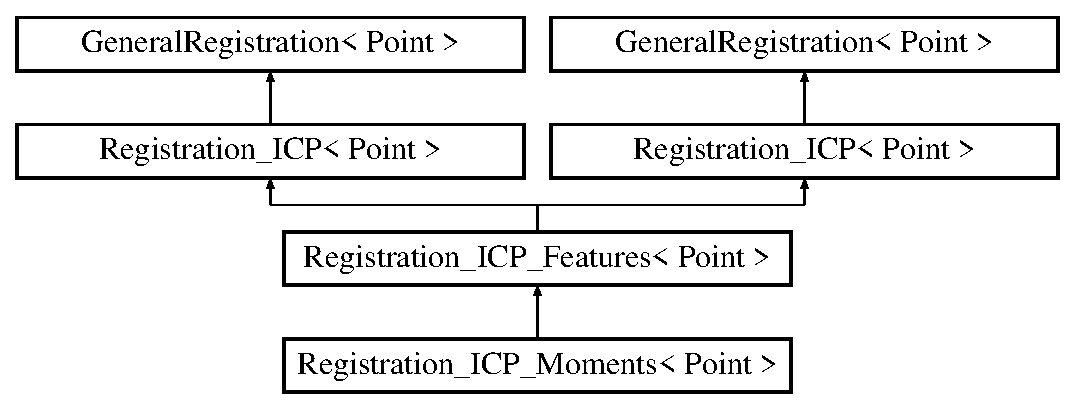
\includegraphics[height=4.000000cm]{classRegistration__ICP__Moments}
\end{center}
\end{figure}
\subsection*{Public Member Functions}
\begin{DoxyCompactItemize}
\item 
\hypertarget{classRegistration__ICP__Moments_a8c90e2d906e9a1ce411ffd07ec76de74}{
void {\bfseries setMomentRadius} (float v)}
\label{classRegistration__ICP__Moments_a8c90e2d906e9a1ce411ffd07ec76de74}

\end{DoxyCompactItemize}
\subsection*{Protected Member Functions}
\begin{DoxyCompactItemize}
\item 
\hypertarget{classRegistration__ICP__Moments_afbdef80f70c26b3cb6843144cc48a36a}{
virtual bool {\bfseries compute\_\-features} ()}
\label{classRegistration__ICP__Moments_afbdef80f70c26b3cb6843144cc48a36a}

\end{DoxyCompactItemize}
\subsubsection*{template$<$typename Point$>$ class Registration\_\-ICP\_\-Moments$<$ Point $>$}



The documentation for this class was generated from the following file:\begin{DoxyCompactItemize}
\item 
common/include/registration/registration\_\-icp\_\-moments.h\end{DoxyCompactItemize}

\hypertarget{classRegistration__ICP__NARF}{
\section{Registration\_\-ICP\_\-NARF$<$ Point $>$ Class Template Reference}
\label{classRegistration__ICP__NARF}\index{Registration\_\-ICP\_\-NARF@{Registration\_\-ICP\_\-NARF}}
}
Inheritance diagram for Registration\_\-ICP\_\-NARF$<$ Point $>$:\begin{figure}[H]
\begin{center}
\leavevmode
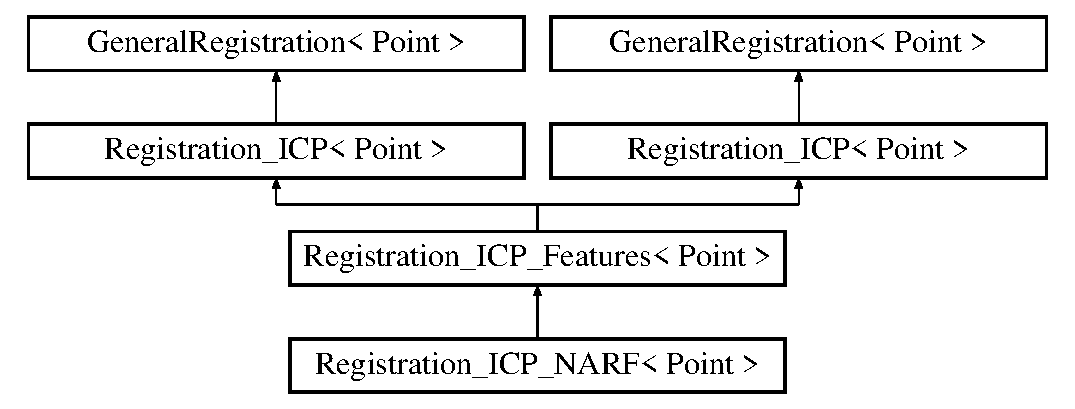
\includegraphics[height=4.000000cm]{classRegistration__ICP__NARF}
\end{center}
\end{figure}
\subsection*{Public Member Functions}
\begin{DoxyCompactItemize}
\item 
\hypertarget{classRegistration__ICP__NARF_ae0aeb380bf05e1d7d58c5c690a97bdfe}{
virtual boost::shared\_\-ptr$<$ const pcl::PointCloud$<$ Point $>$ $>$ \hyperlink{classRegistration__ICP__NARF_ae0aeb380bf05e1d7d58c5c690a97bdfe}{getMarkers} ()}
\label{classRegistration__ICP__NARF_ae0aeb380bf05e1d7d58c5c690a97bdfe}

\begin{DoxyCompactList}\small\item\em debug function for marker visualization \item\end{DoxyCompactList}\end{DoxyCompactItemize}
\subsection*{Protected Member Functions}
\begin{DoxyCompactItemize}
\item 
\hypertarget{classRegistration__ICP__NARF_af3a81b95182d0a3220293eb4d88bf78b}{
virtual bool {\bfseries compute\_\-features} ()}
\label{classRegistration__ICP__NARF_af3a81b95182d0a3220293eb4d88bf78b}

\item 
\hypertarget{classRegistration__ICP__NARF_aabcabb41826a7ef97fc2f9709312ab5d}{
virtual bool {\bfseries compute\_\-transformation} ()}
\label{classRegistration__ICP__NARF_aabcabb41826a7ef97fc2f9709312ab5d}

\end{DoxyCompactItemize}
\subsubsection*{template$<$typename Point$>$ class Registration\_\-ICP\_\-NARF$<$ Point $>$}



The documentation for this class was generated from the following file:\begin{DoxyCompactItemize}
\item 
common/include/registration/registration\_\-icp\_\-narf.h\end{DoxyCompactItemize}

\hypertarget{classRegistration__Infobased}{
\section{Registration\_\-Infobased$<$ Point $>$ Class Template Reference}
\label{classRegistration__Infobased}\index{Registration\_\-Infobased@{Registration\_\-Infobased}}
}
Inheritance diagram for Registration\_\-Infobased$<$ Point $>$:\begin{figure}[H]
\begin{center}
\leavevmode
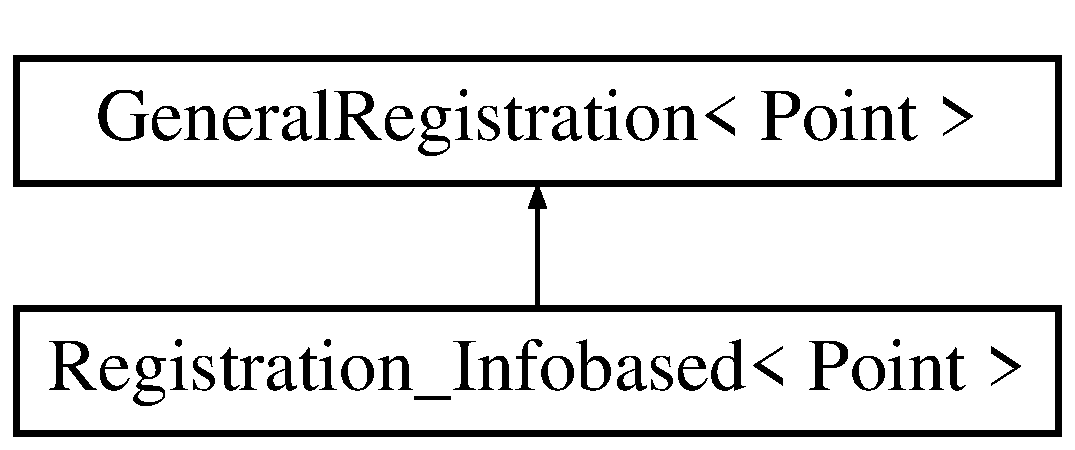
\includegraphics[height=2.000000cm]{classRegistration__Infobased}
\end{center}
\end{figure}
\subsection*{Public Member Functions}
\begin{DoxyCompactItemize}
\item 
\hypertarget{classRegistration__Infobased_a8736c7e147dfe0e1970745946c84572e}{
void {\bfseries setUseICP} (const bool b)}
\label{classRegistration__Infobased_a8736c7e147dfe0e1970745946c84572e}

\item 
\hypertarget{classRegistration__Infobased_a5780a16f8e3117f2f0fcba6689daec04}{
virtual boost::shared\_\-ptr$<$ pcl::PointCloud$<$ Point $>$ $>$ \hyperlink{classRegistration__Infobased_a5780a16f8e3117f2f0fcba6689daec04}{getMap} ()}
\label{classRegistration__Infobased_a5780a16f8e3117f2f0fcba6689daec04}

\begin{DoxyCompactList}\small\item\em map is not necessarily implemented \item\end{DoxyCompactList}\item 
\hypertarget{classRegistration__Infobased_ae08c19be51f80cb68fa6de0dca888a88}{
pcl::PointCloud$<$ Point $>$ \& {\bfseries getSource} ()}
\label{classRegistration__Infobased_ae08c19be51f80cb68fa6de0dca888a88}

\item 
\hypertarget{classRegistration__Infobased_a22635c046c5678769d14fcb7356a347f}{
pcl::PointCloud$<$ Point $>$ \& {\bfseries getTarget} ()}
\label{classRegistration__Infobased_a22635c046c5678769d14fcb7356a347f}

\item 
\hypertarget{classRegistration__Infobased_a130f9051bbfeda57d765e919ea8870e0}{
virtual boost::shared\_\-ptr$<$ const pcl::PointCloud$<$ Point $>$ $>$ \hyperlink{classRegistration__Infobased_a130f9051bbfeda57d765e919ea8870e0}{getMarkers} ()}
\label{classRegistration__Infobased_a130f9051bbfeda57d765e919ea8870e0}

\begin{DoxyCompactList}\small\item\em debug function for marker visualization \item\end{DoxyCompactList}\end{DoxyCompactItemize}
\subsection*{Protected Member Functions}
\begin{DoxyCompactItemize}
\item 
\hypertarget{classRegistration__Infobased_ab016a8a196669659952729589e8f9c5f}{
virtual bool {\bfseries compute\_\-features} ()}
\label{classRegistration__Infobased_ab016a8a196669659952729589e8f9c5f}

\item 
\hypertarget{classRegistration__Infobased_a6f7b7249d32b0f2f76052d2cbbf8f63e}{
virtual bool {\bfseries compute\_\-corrospondences} ()}
\label{classRegistration__Infobased_a6f7b7249d32b0f2f76052d2cbbf8f63e}

\item 
\hypertarget{classRegistration__Infobased_ac3bd2459aa5b39223aa0faba283f1dc2}{
virtual bool {\bfseries compute\_\-transformation} ()}
\label{classRegistration__Infobased_ac3bd2459aa5b39223aa0faba283f1dc2}

\item 
\hypertarget{classRegistration__Infobased_ac7d1ecf11333c36537d719f96d00b5be}{
float {\bfseries getMaxDiff2} (const pcl::PointCloud$<$ Point $>$ \&pc, const int ind, const pcl::PointCloud$<$ Point $>$ \&pc2, int \&mi)}
\label{classRegistration__Infobased_ac7d1ecf11333c36537d719f96d00b5be}

\item 
\hypertarget{classRegistration__Infobased_a892c4ad907ee8bd98dcc102d89b784ec}{
float {\bfseries getMaxDiff} (const pcl::PointCloud$<$ Point $>$ \&pc, const int ind)}
\label{classRegistration__Infobased_a892c4ad907ee8bd98dcc102d89b784ec}

\item 
\hypertarget{classRegistration__Infobased_aaf9398c5d32e26895c6e14684fb74380}{
int {\bfseries getI} (const int ind, const pcl::PointCloud$<$ Point $>$ \&pc)}
\label{classRegistration__Infobased_aaf9398c5d32e26895c6e14684fb74380}

\item 
\hypertarget{classRegistration__Infobased_a1c553bcad88092d5c1d1ddcf39a128b8}{
float {\bfseries findCorr} (pcl::PointCloud$<$ Point $>$ \&pc\_\-old, const pcl::PointCloud$<$ Point $>$ \&pc\_\-new, std::vector$<$ int $>$ \&cor\_\-inds)}
\label{classRegistration__Infobased_a1c553bcad88092d5c1d1ddcf39a128b8}

\item 
\hypertarget{classRegistration__Infobased_ae1e5447da4c02579fc2186a254c0577c}{
void {\bfseries getDis} (const Eigen::Vector3f \&C, const Eigen::Vector3f \&S, float \&dT, float \&dA)}
\label{classRegistration__Infobased_ae1e5447da4c02579fc2186a254c0577c}

\item 
\hypertarget{classRegistration__Infobased_acbff89b4a2cd7e2f1c1b1b34b0cb8dd9}{
float {\bfseries calc\_\-error} (const pcl::PointCloud$<$ Point $>$ \&s, const pcl::PointCloud$<$ Point $>$ \&t)}
\label{classRegistration__Infobased_acbff89b4a2cd7e2f1c1b1b34b0cb8dd9}

\end{DoxyCompactItemize}
\subsection*{Protected Attributes}
\begin{DoxyCompactItemize}
\item 
\hypertarget{classRegistration__Infobased_a9a316bf088021afaada65470673cf7c4}{
pcl::PointCloud$<$ Point $>$ {\bfseries register\_\-}}
\label{classRegistration__Infobased_a9a316bf088021afaada65470673cf7c4}

\item 
\hypertarget{classRegistration__Infobased_a093d3ca42b8511a984f81d13346fd318}{
pcl::PointCloud$<$ Point $>$ {\bfseries markers\_\-}}
\label{classRegistration__Infobased_a093d3ca42b8511a984f81d13346fd318}

\end{DoxyCompactItemize}
\subsubsection*{template$<$typename Point$>$ class Registration\_\-Infobased$<$ Point $>$}



The documentation for this class was generated from the following files:\begin{DoxyCompactItemize}
\item 
common/include/registration/registration\_\-info.h\item 
common/include/registration/impl/registration\_\-info.hpp\end{DoxyCompactItemize}

\hypertarget{classRegistration__RGBDSLAM}{
\section{Registration\_\-RGBDSLAM$<$ Point $>$ Class Template Reference}
\label{classRegistration__RGBDSLAM}\index{Registration\_\-RGBDSLAM@{Registration\_\-RGBDSLAM}}
}


{\ttfamily \#include $<$registration\_\-rgbdslam.h$>$}

Inheritance diagram for Registration\_\-RGBDSLAM$<$ Point $>$:\begin{figure}[H]
\begin{center}
\leavevmode
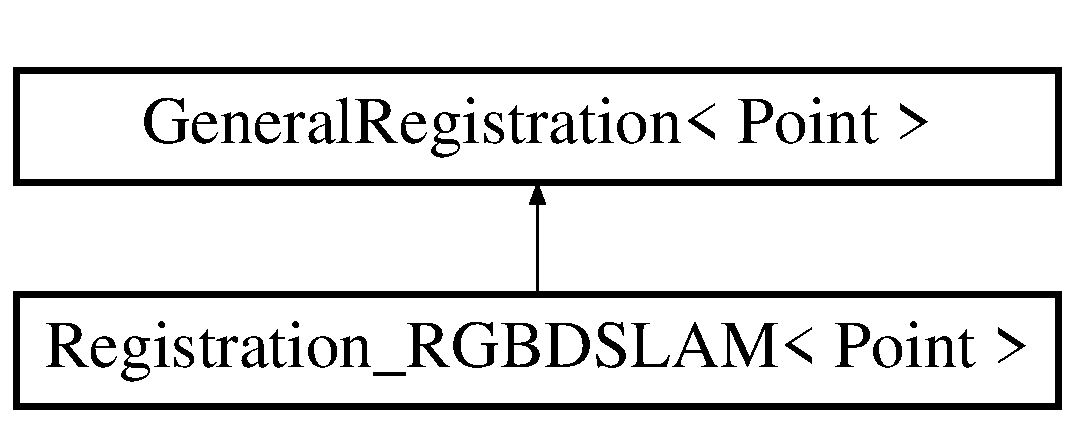
\includegraphics[height=2.000000cm]{classRegistration__RGBDSLAM}
\end{center}
\end{figure}
\subsection*{Public Member Functions}
\begin{DoxyCompactItemize}
\item 
\hypertarget{classRegistration__RGBDSLAM_ab2bfaca24dc1d7c02bb512c4ead4d939}{
{\bfseries Registration\_\-RGBDSLAM} (ros::NodeHandle \&nh)}
\label{classRegistration__RGBDSLAM_ab2bfaca24dc1d7c02bb512c4ead4d939}

\item 
\hypertarget{classRegistration__RGBDSLAM_a119c92ef6613c9bea7d7507559974178}{
boost::shared\_\-ptr$<$ pcl::PointCloud$<$ Point $>$ $>$ \hyperlink{classRegistration__RGBDSLAM_a119c92ef6613c9bea7d7507559974178}{getMap} ()}
\label{classRegistration__RGBDSLAM_a119c92ef6613c9bea7d7507559974178}

\begin{DoxyCompactList}\small\item\em map is not necessarily implemented \item\end{DoxyCompactList}\end{DoxyCompactItemize}
\subsection*{Protected Member Functions}
\begin{DoxyCompactItemize}
\item 
\hypertarget{classRegistration__RGBDSLAM_a4160e4cbc8a7cfeda378e9da0495618d}{
virtual bool {\bfseries compute\_\-features} ()}
\label{classRegistration__RGBDSLAM_a4160e4cbc8a7cfeda378e9da0495618d}

\item 
\hypertarget{classRegistration__RGBDSLAM_ad9156fba578117effbb54669808df3fa}{
virtual bool {\bfseries compute\_\-corrospondences} ()}
\label{classRegistration__RGBDSLAM_ad9156fba578117effbb54669808df3fa}

\item 
\hypertarget{classRegistration__RGBDSLAM_a9a57f40c068a98520efb4401fb07f0e0}{
virtual bool {\bfseries compute\_\-transformation} ()}
\label{classRegistration__RGBDSLAM_a9a57f40c068a98520efb4401fb07f0e0}

\item 
\hypertarget{classRegistration__RGBDSLAM_a6d80282ad1d5547295f43a3018ea735b}{
void \hyperlink{classRegistration__RGBDSLAM_a6d80282ad1d5547295f43a3018ea735b}{transformationCallback} (const tf::tfMessage \&transform)}
\label{classRegistration__RGBDSLAM_a6d80282ad1d5547295f43a3018ea735b}

\begin{DoxyCompactList}\small\item\em get last transformation and calculate the transformation matrix \item\end{DoxyCompactList}\end{DoxyCompactItemize}
\subsection*{Protected Attributes}
\begin{DoxyCompactItemize}
\item 
\hypertarget{classRegistration__RGBDSLAM_a32d5fe77a83e546080aaee1bcdead42f}{
pcl::PointCloud$<$ Point $>$ {\bfseries register\_\-}}
\label{classRegistration__RGBDSLAM_a32d5fe77a83e546080aaee1bcdead42f}

\item 
\hypertarget{classRegistration__RGBDSLAM_af83c679733a4eef87053200ec583fa72}{
ros::Publisher {\bfseries pub\_\-img\_\-}}
\label{classRegistration__RGBDSLAM_af83c679733a4eef87053200ec583fa72}

\item 
\hypertarget{classRegistration__RGBDSLAM_a163812fdfbaeb9b8db3f59c05ee00663}{
ros::Publisher {\bfseries pub\_\-img\_\-depth\_\-}}
\label{classRegistration__RGBDSLAM_a163812fdfbaeb9b8db3f59c05ee00663}

\item 
\hypertarget{classRegistration__RGBDSLAM_a31a5dc9b215fa9157cb890d84bf3cfbc}{
ros::Publisher {\bfseries pub\_\-camera\_\-info\_\-}}
\label{classRegistration__RGBDSLAM_a31a5dc9b215fa9157cb890d84bf3cfbc}

\item 
\hypertarget{classRegistration__RGBDSLAM_a0d2001a54b8013b602004a892cab4249}{
ros::Publisher {\bfseries pub\_\-cloud\_\-}}
\label{classRegistration__RGBDSLAM_a0d2001a54b8013b602004a892cab4249}

\item 
\hypertarget{classRegistration__RGBDSLAM_a0c92e217d23b31dfb1add3e652dba29a}{
ros::Subscriber {\bfseries sub\_\-trans\_\-}}
\label{classRegistration__RGBDSLAM_a0c92e217d23b31dfb1add3e652dba29a}

\end{DoxyCompactItemize}


\subsection{Detailed Description}
\subsubsection*{template$<$typename Point$>$ class Registration\_\-RGBDSLAM$<$ Point $>$}

class which wraps the interface to rgbd slam

topics needed:
\begin{DoxyItemize}
\item /camera/rgb/image\_\-mono
\item /camera/depth/image
\item /camera/rgb/camera\_\-info
\item /camera/rgb/points topics output:
\item /rgbdslam/cloud
\item /rgbdslam/transformed\_\-slowdown\_\-cloud
\item /rgbdslam/first\_\-frame
\item /rgbdslam/transforms 
\end{DoxyItemize}

The documentation for this class was generated from the following files:\begin{DoxyCompactItemize}
\item 
ros/include/registration\_\-rgbdslam.h\item 
ros/include/impl/registration\_\-rgbdslam.hpp\end{DoxyCompactItemize}

\hypertarget{classRegistrationNode}{
\section{RegistrationNode Class Reference}
\label{classRegistrationNode}\index{RegistrationNode@{RegistrationNode}}
}
\subsection*{Public Member Functions}
\begin{DoxyCompactItemize}
\item 
\hypertarget{classRegistrationNode_a4d2461773d8a8736556c5a14e22ead39}{
{\bfseries RegistrationNode} (bool dummy)}
\label{classRegistrationNode_a4d2461773d8a8736556c5a14e22ead39}

\item 
\hyperlink{classRegistrationNode_a061d1dd7a7d20ce2f6f1b49effc242f7}{$\sim$RegistrationNode} ()
\item 
void \hyperlink{classRegistrationNode_a088465f420639938a06747c8ee4c4df7}{onInit} ()
\begin{DoxyCompactList}\small\item\em initializes parameters \item\end{DoxyCompactList}\item 
void \hyperlink{classRegistrationNode_aa4c32460d529b455cd3a8f264e379ecb}{createParamters} (const std::string \&algo)
\item 
void \hyperlink{classRegistrationNode_a314ac88efd6a9165c5db16de31a68496}{publishParameters} ()
\item 
void \hyperlink{classRegistrationNode_a7da9e7d7af487ba6760e656b6a9790a4}{buildAlgo} ()
\item 
void \hyperlink{classRegistrationNode_ad58ddd35fc39f760197225500100ac30}{pointCloudSubCallback} (const pcl::PointCloud$<$ Point $>$::Ptr \&pc\_\-in)
\begin{DoxyCompactList}\small\item\em callback for point cloud subroutine \item\end{DoxyCompactList}\item 
bool \hyperlink{classRegistrationNode_a83816fd7a40b43b04a76c4e71995d215}{registerService} (::registration::RegistrationPCD::Request \&req,::registration::RegistrationPCD::Response \&res)
\end{DoxyCompactItemize}
\subsection*{Public Attributes}
\begin{DoxyCompactItemize}
\item 
\hypertarget{classRegistrationNode_ad756391e2bcbae371580c09249fb9277}{
ros::NodeHandle {\bfseries n\_\-}}
\label{classRegistrationNode_ad756391e2bcbae371580c09249fb9277}

\item 
\hypertarget{classRegistrationNode_a97206aeb3f84ce6ec1d92c2bafa55ca9}{
ros::Time {\bfseries stamp\_\-}}
\label{classRegistrationNode_a97206aeb3f84ce6ec1d92c2bafa55ca9}

\end{DoxyCompactItemize}
\subsection*{Protected Types}
\begin{DoxyCompactItemize}
\item 
enum \{ \par
{\bfseries E\_\-ALGO\_\-ICP} = 1, 
{\bfseries E\_\-ALGO\_\-ICP\_\-LM} = 2, 
{\bfseries E\_\-ALGO\_\-GICP} = 3, 
{\bfseries E\_\-ALGO\_\-ICP\_\-MOMENTS} = 4, 
\par
{\bfseries E\_\-ALGO\_\-ICP\_\-FPFH} = 5, 
{\bfseries E\_\-ALGO\_\-ICP\_\-NARF} = 6, 
{\bfseries E\_\-ALGO\_\-FASTSLAM} = 7, 
{\bfseries E\_\-ALGO\_\-ICP\_\-EDGES} = 8, 
\par
{\bfseries E\_\-ALGO\_\-RGBDSLAM} = 9, 
{\bfseries E\_\-ALGO\_\-INFO} = 10, 
{\bfseries E\_\-ALGO\_\-COR} = 11, 
{\bfseries E\_\-ALGO\_\-NONE} = 0
 \}
\end{DoxyCompactItemize}
\subsection*{Protected Member Functions}
\begin{DoxyCompactItemize}
\item 
void \hyperlink{classRegistrationNode_a4c014e25b84d541c26b381d7c163f9f4}{publish\_\-results} ()
\item 
bool \hyperlink{classRegistrationNode_a49613a1b302f646f7e222c0daa1a9e7b}{do\_\-preprocess} (pcl::PointCloud$<$ Point $>$ \&pc, cv\_\-bridge::CvImagePtr \&cv\_\-ptr, cv::Mat \&img\_\-depth)
\item 
bool \hyperlink{classRegistrationNode_a4c57bd480d76df5ab6b186a6521d1822}{do\_\-register} (const pcl::PointCloud$<$ Point $>$ \&pc, const cv\_\-bridge::CvImagePtr \&cv\_\-ptr, cv::Mat \&img\_\-depth)
\item 
\hypertarget{classRegistrationNode_ad37f0db5fd52b870426794d2b44cef08}{
void {\bfseries setSettings\_\-ICP} (\hyperlink{classRegistration__ICP}{Registration\_\-ICP}$<$ Point $>$ $\ast$pr)}
\label{classRegistrationNode_ad37f0db5fd52b870426794d2b44cef08}

\item 
\hypertarget{classRegistrationNode_aaf68c48a76890081dd89ffecb9d6c1c7}{
void {\bfseries setSettings\_\-ICP\_\-Moments} (\hyperlink{classRegistration__ICP__Moments}{Registration\_\-ICP\_\-Moments}$<$ Point $>$ $\ast$pr)}
\label{classRegistrationNode_aaf68c48a76890081dd89ffecb9d6c1c7}

\item 
\hypertarget{classRegistrationNode_a82d75e7f4013b917ce3e1f57b12e87e8}{
void {\bfseries setSettings\_\-ICP\_\-FPFH} (\hyperlink{classRegistration__ICP__FPFH}{Registration\_\-ICP\_\-FPFH}$<$ Point $>$ $\ast$pr)}
\label{classRegistrationNode_a82d75e7f4013b917ce3e1f57b12e87e8}

\item 
\hypertarget{classRegistrationNode_a924764ad64859741ebe4a8e1070f08a9}{
void {\bfseries setSettings\_\-ICP\_\-NARF} (\hyperlink{classRegistration__ICP__NARF}{Registration\_\-ICP\_\-NARF}$<$ Point $>$ $\ast$pr)}
\label{classRegistrationNode_a924764ad64859741ebe4a8e1070f08a9}

\item 
\hypertarget{classRegistrationNode_a4929fcef285c47872eb412b99a5a6286}{
void {\bfseries setSettings\_\-ICP\_\-Edges} (\hyperlink{classRegistration__ICP__Edges}{Registration\_\-ICP\_\-Edges}$<$ Point $>$ $\ast$pr)}
\label{classRegistrationNode_a4929fcef285c47872eb412b99a5a6286}

\item 
\hypertarget{classRegistrationNode_a4e62d689b604dcc07a90738a48eeb112}{
void {\bfseries setSettings\_\-Info} (\hyperlink{classRegistration__Infobased}{Registration\_\-Infobased}$<$ Point $>$ $\ast$pr)}
\label{classRegistrationNode_a4e62d689b604dcc07a90738a48eeb112}

\item 
\hypertarget{classRegistrationNode_aace7037e3ac43e5d2925f2a5ae9b7248}{
void {\bfseries publishMarkerPoint} (const Point \&p, int id, float r, float g, float b, float Size=0.02)}
\label{classRegistrationNode_aace7037e3ac43e5d2925f2a5ae9b7248}

\item 
\hypertarget{classRegistrationNode_a5329c6053bf5b9a9e4e6d444612efaa1}{
void {\bfseries publishLineMarker} (Eigen::Vector3f a, Eigen::Vector3f b, const int id=rand()\%111111)}
\label{classRegistrationNode_a5329c6053bf5b9a9e4e6d444612efaa1}

\end{DoxyCompactItemize}
\subsection*{Protected Attributes}
\begin{DoxyCompactItemize}
\item 
\hypertarget{classRegistrationNode_ad13d7e29d9a11fbe33705207856828b7}{
ros::Subscriber {\bfseries point\_\-cloud\_\-sub\_\-}}
\label{classRegistrationNode_ad13d7e29d9a11fbe33705207856828b7}

\item 
\hypertarget{classRegistrationNode_ae5d6a5bc2cba20991dad627df98e40df}{
ros::ServiceServer \hyperlink{classRegistrationNode_ae5d6a5bc2cba20991dad627df98e40df}{register\_\-ser\_\-}}
\label{classRegistrationNode_ae5d6a5bc2cba20991dad627df98e40df}

\begin{DoxyCompactList}\small\item\em subscriber to input data \item\end{DoxyCompactList}\item 
\hypertarget{classRegistrationNode_a9e32e3410a5df73d604b7fc2771b2d7a}{
TransformListener \hyperlink{classRegistrationNode_a9e32e3410a5df73d604b7fc2771b2d7a}{tf\_\-listener\_\-}}
\label{classRegistrationNode_a9e32e3410a5df73d604b7fc2771b2d7a}

\begin{DoxyCompactList}\small\item\em service for evaluation of registration \item\end{DoxyCompactList}\item 
\hypertarget{classRegistrationNode_a6d3cdad1532c2dc263060938bbd81aed}{
ros::Publisher {\bfseries point\_\-cloud\_\-pub\_\-}}
\label{classRegistrationNode_a6d3cdad1532c2dc263060938bbd81aed}

\item 
\hypertarget{classRegistrationNode_a11653721623a3641d0279011664d829b}{
ros::Publisher \hyperlink{classRegistrationNode_a11653721623a3641d0279011664d829b}{marker\_\-pub\_\-}}
\label{classRegistrationNode_a11653721623a3641d0279011664d829b}

\begin{DoxyCompactList}\small\item\em publisher for map \item\end{DoxyCompactList}\item 
\hyperlink{classParameterBucket}{ParameterBucket} \hyperlink{classRegistrationNode_a64f206a310aa231161d13fd7aa54380d}{parameters\_\-}
\begin{DoxyCompactList}\small\item\em publish markers for visualization \item\end{DoxyCompactList}\item 
\hypertarget{classRegistrationNode_af89c036128385228f4d74fc5908803e8}{
\hyperlink{classGeneralRegistration}{GeneralRegistration}$<$ Point $>$ $\ast$ \hyperlink{classRegistrationNode_af89c036128385228f4d74fc5908803e8}{reg\_\-}}
\label{classRegistrationNode_af89c036128385228f4d74fc5908803e8}

\begin{DoxyCompactList}\small\item\em registration algorithm \item\end{DoxyCompactList}\item 
\hypertarget{classRegistrationNode_af51e29db4f2f9abcedcb8a1c43396838}{
double \hyperlink{classRegistrationNode_af51e29db4f2f9abcedcb8a1c43396838}{duration\_\-}}
\label{classRegistrationNode_af51e29db4f2f9abcedcb8a1c43396838}

\begin{DoxyCompactList}\small\item\em evaluation: duration in seconds \item\end{DoxyCompactList}\item 
\hypertarget{classRegistrationNode_a8ae0191181e275268c82182c828e1842}{
int \hyperlink{classRegistrationNode_a8ae0191181e275268c82182c828e1842}{memory\_\-usage\_\-kb\_\-}}
\label{classRegistrationNode_a8ae0191181e275268c82182c828e1842}

\begin{DoxyCompactList}\small\item\em evaluation: incremental memory usage in kB \item\end{DoxyCompactList}\item 
\hypertarget{classRegistrationNode_a4630d8b7a3c1816e672f82897f3989b8}{
bool \hyperlink{classRegistrationNode_a4630d8b7a3c1816e672f82897f3989b8}{registration\_\-result\_\-}}
\label{classRegistrationNode_a4630d8b7a3c1816e672f82897f3989b8}

\begin{DoxyCompactList}\small\item\em evaluation: success -\/$>$ true \item\end{DoxyCompactList}\end{DoxyCompactItemize}


\subsection{Constructor \& Destructor Documentation}
\hypertarget{classRegistrationNode_a061d1dd7a7d20ce2f6f1b49effc242f7}{
\index{RegistrationNode@{RegistrationNode}!$\sim$RegistrationNode@{$\sim$RegistrationNode}}
\index{$\sim$RegistrationNode@{$\sim$RegistrationNode}!RegistrationNode@{RegistrationNode}}
\subsubsection[{$\sim$RegistrationNode}]{\setlength{\rightskip}{0pt plus 5cm}RegistrationNode::$\sim$RegistrationNode (
\begin{DoxyParamCaption}
{}
\end{DoxyParamCaption}
)\hspace{0.3cm}{\ttfamily  \mbox{[}inline\mbox{]}}}}
\label{classRegistrationNode_a061d1dd7a7d20ce2f6f1b49effc242f7}


void 



\subsection{Member Function Documentation}
\hypertarget{classRegistrationNode_a7da9e7d7af487ba6760e656b6a9790a4}{
\index{RegistrationNode@{RegistrationNode}!buildAlgo@{buildAlgo}}
\index{buildAlgo@{buildAlgo}!RegistrationNode@{RegistrationNode}}
\subsubsection[{buildAlgo}]{\setlength{\rightskip}{0pt plus 5cm}void RegistrationNode::buildAlgo (
\begin{DoxyParamCaption}
{}
\end{DoxyParamCaption}
)\hspace{0.3cm}{\ttfamily  \mbox{[}inline\mbox{]}}}}
\label{classRegistrationNode_a7da9e7d7af487ba6760e656b6a9790a4}
reading out parameter and creating an instance of the algorithm setting all needed parameters for algorithm \hypertarget{classRegistrationNode_aa4c32460d529b455cd3a8f264e379ecb}{
\index{RegistrationNode@{RegistrationNode}!createParamters@{createParamters}}
\index{createParamters@{createParamters}!RegistrationNode@{RegistrationNode}}
\subsubsection[{createParamters}]{\setlength{\rightskip}{0pt plus 5cm}void RegistrationNode::createParamters (
\begin{DoxyParamCaption}
\item[{const std::string \&}]{ algo}
\end{DoxyParamCaption}
)\hspace{0.3cm}{\ttfamily  \mbox{[}inline\mbox{]}}}}
\label{classRegistrationNode_aa4c32460d529b455cd3a8f264e379ecb}
creating parameter settings for evaluation it's not thought to be used for registration self \hypertarget{classRegistrationNode_a49613a1b302f646f7e222c0daa1a9e7b}{
\index{RegistrationNode@{RegistrationNode}!do\_\-preprocess@{do\_\-preprocess}}
\index{do\_\-preprocess@{do\_\-preprocess}!RegistrationNode@{RegistrationNode}}
\subsubsection[{do\_\-preprocess}]{\setlength{\rightskip}{0pt plus 5cm}bool RegistrationNode::do\_\-preprocess (
\begin{DoxyParamCaption}
\item[{pcl::PointCloud$<$ Point $>$ \&}]{ pc, }
\item[{cv\_\-bridge::CvImagePtr \&}]{ cv\_\-ptr, }
\item[{cv::Mat \&}]{ img\_\-depth}
\end{DoxyParamCaption}
)\hspace{0.3cm}{\ttfamily  \mbox{[}inline, protected\mbox{]}}}}
\label{classRegistrationNode_a49613a1b302f646f7e222c0daa1a9e7b}
preprocessing data \hypertarget{classRegistrationNode_a4c57bd480d76df5ab6b186a6521d1822}{
\index{RegistrationNode@{RegistrationNode}!do\_\-register@{do\_\-register}}
\index{do\_\-register@{do\_\-register}!RegistrationNode@{RegistrationNode}}
\subsubsection[{do\_\-register}]{\setlength{\rightskip}{0pt plus 5cm}bool RegistrationNode::do\_\-register (
\begin{DoxyParamCaption}
\item[{const pcl::PointCloud$<$ Point $>$ \&}]{ pc, }
\item[{const cv\_\-bridge::CvImagePtr \&}]{ cv\_\-ptr, }
\item[{cv::Mat \&}]{ img\_\-depth}
\end{DoxyParamCaption}
)\hspace{0.3cm}{\ttfamily  \mbox{[}inline, protected\mbox{]}}}}
\label{classRegistrationNode_a4c57bd480d76df5ab6b186a6521d1822}
registration process
\begin{DoxyItemize}
\item setting input data
\item measurement
\item visualization helper (for debugging) 
\end{DoxyItemize}\hypertarget{classRegistrationNode_a088465f420639938a06747c8ee4c4df7}{
\index{RegistrationNode@{RegistrationNode}!onInit@{onInit}}
\index{onInit@{onInit}!RegistrationNode@{RegistrationNode}}
\subsubsection[{onInit}]{\setlength{\rightskip}{0pt plus 5cm}void RegistrationNode::onInit (
\begin{DoxyParamCaption}
{}
\end{DoxyParamCaption}
)\hspace{0.3cm}{\ttfamily  \mbox{[}inline\mbox{]}}}}
\label{classRegistrationNode_a088465f420639938a06747c8ee4c4df7}


initializes parameters 

initializes parameters

\begin{DoxyReturn}{Returns}
nothing 
\end{DoxyReturn}
\hypertarget{classRegistrationNode_ad58ddd35fc39f760197225500100ac30}{
\index{RegistrationNode@{RegistrationNode}!pointCloudSubCallback@{pointCloudSubCallback}}
\index{pointCloudSubCallback@{pointCloudSubCallback}!RegistrationNode@{RegistrationNode}}
\subsubsection[{pointCloudSubCallback}]{\setlength{\rightskip}{0pt plus 5cm}void RegistrationNode::pointCloudSubCallback (
\begin{DoxyParamCaption}
\item[{const pcl::PointCloud$<$ Point $>$::Ptr \&}]{ pc\_\-in}
\end{DoxyParamCaption}
)\hspace{0.3cm}{\ttfamily  \mbox{[}inline\mbox{]}}}}
\label{classRegistrationNode_ad58ddd35fc39f760197225500100ac30}


callback for point cloud subroutine 

callback for point cloud subroutine which stores the point cloud for further calculation


\begin{DoxyParams}{Parameters}
\item[{\em pc\_\-in}]new point cloud\end{DoxyParams}
\begin{DoxyReturn}{Returns}
nothing 
\end{DoxyReturn}
\hypertarget{classRegistrationNode_a4c014e25b84d541c26b381d7c163f9f4}{
\index{RegistrationNode@{RegistrationNode}!publish\_\-results@{publish\_\-results}}
\index{publish\_\-results@{publish\_\-results}!RegistrationNode@{RegistrationNode}}
\subsubsection[{publish\_\-results}]{\setlength{\rightskip}{0pt plus 5cm}void RegistrationNode::publish\_\-results (
\begin{DoxyParamCaption}
{}
\end{DoxyParamCaption}
)\hspace{0.3cm}{\ttfamily  \mbox{[}inline, protected\mbox{]}}}}
\label{classRegistrationNode_a4c014e25b84d541c26b381d7c163f9f4}
publishing evaluation results \hypertarget{classRegistrationNode_a314ac88efd6a9165c5db16de31a68496}{
\index{RegistrationNode@{RegistrationNode}!publishParameters@{publishParameters}}
\index{publishParameters@{publishParameters}!RegistrationNode@{RegistrationNode}}
\subsubsection[{publishParameters}]{\setlength{\rightskip}{0pt plus 5cm}void RegistrationNode::publishParameters (
\begin{DoxyParamCaption}
{}
\end{DoxyParamCaption}
)\hspace{0.3cm}{\ttfamily  \mbox{[}inline\mbox{]}}}}
\label{classRegistrationNode_a314ac88efd6a9165c5db16de31a68496}
reading out all parameters from parameter bag and publishing them as parameterlist thought to be used for evaluation \hypertarget{classRegistrationNode_a83816fd7a40b43b04a76c4e71995d215}{
\index{RegistrationNode@{RegistrationNode}!registerService@{registerService}}
\index{registerService@{registerService}!RegistrationNode@{RegistrationNode}}
\subsubsection[{registerService}]{\setlength{\rightskip}{0pt plus 5cm}bool RegistrationNode::registerService (
\begin{DoxyParamCaption}
\item[{::registration::RegistrationPCD::Request \&}]{ req, }
\item[{::registration::RegistrationPCD::Response \&}]{ res}
\end{DoxyParamCaption}
)\hspace{0.3cm}{\ttfamily  \mbox{[}inline\mbox{]}}}}
\label{classRegistrationNode_a83816fd7a40b43b04a76c4e71995d215}
service callback to register a dataset returning success 

\subsection{Member Data Documentation}
\hypertarget{classRegistrationNode_a64f206a310aa231161d13fd7aa54380d}{
\index{RegistrationNode@{RegistrationNode}!parameters\_\-@{parameters\_\-}}
\index{parameters\_\-@{parameters\_\-}!RegistrationNode@{RegistrationNode}}
\subsubsection[{parameters\_\-}]{\setlength{\rightskip}{0pt plus 5cm}{\bf ParameterBucket} {\bf RegistrationNode::parameters\_\-}\hspace{0.3cm}{\ttfamily  \mbox{[}protected\mbox{]}}}}
\label{classRegistrationNode_a64f206a310aa231161d13fd7aa54380d}


publish markers for visualization 

parameter bag (containing max, min, step...) 

The documentation for this class was generated from the following file:\begin{DoxyCompactItemize}
\item 
ros/src/registration\_\-node.cpp\end{DoxyCompactItemize}

\hypertarget{classRegKeypointCorrespondence}{
\section{RegKeypointCorrespondence$<$ Point, Keypoint $>$ Class Template Reference}
\label{classRegKeypointCorrespondence}\index{RegKeypointCorrespondence@{RegKeypointCorrespondence}}
}
Inheritance diagram for RegKeypointCorrespondence$<$ Point, Keypoint $>$:\begin{figure}[H]
\begin{center}
\leavevmode
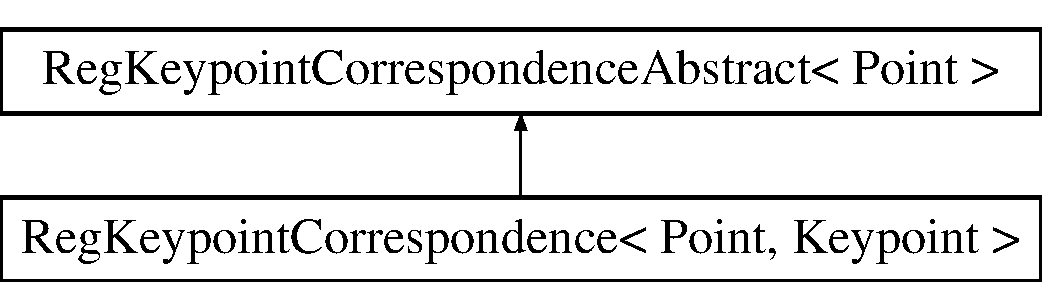
\includegraphics[height=2.000000cm]{classRegKeypointCorrespondence}
\end{center}
\end{figure}
\subsection*{Public Member Functions}
\begin{DoxyCompactItemize}
\item 
\hypertarget{classRegKeypointCorrespondence_a297cfea656d891bea94e2d45245a05d9}{
virtual void {\bfseries getCorrespondences} (std::vector$<$ pcl::registration::Correspondence $>$ \&correspondences)}
\label{classRegKeypointCorrespondence_a297cfea656d891bea94e2d45245a05d9}

\item 
\hypertarget{classRegKeypointCorrespondence_ae055e55096e52385a5a91a6f15bf1fc3}{
virtual boost::shared\_\-ptr$<$ pcl::PointCloud$<$ Point $>$ $>$ {\bfseries getSourcePoints} ()}
\label{classRegKeypointCorrespondence_ae055e55096e52385a5a91a6f15bf1fc3}

\item 
\hypertarget{classRegKeypointCorrespondence_ae43d02fb394fb3e7470ae355ddaa92a1}{
virtual boost::shared\_\-ptr$<$ pcl::PointCloud$<$ Point $>$ $>$ {\bfseries getTargetPoints} ()}
\label{classRegKeypointCorrespondence_ae43d02fb394fb3e7470ae355ddaa92a1}

\end{DoxyCompactItemize}
\subsection*{Protected Member Functions}
\begin{DoxyCompactItemize}
\item 
\hypertarget{classRegKeypointCorrespondence_a045fecfd029e9e4f82ba7ce06a24925d}{
virtual Point {\bfseries getPointForKeypointSrc} (const int ind)=0}
\label{classRegKeypointCorrespondence_a045fecfd029e9e4f82ba7ce06a24925d}

\item 
\hypertarget{classRegKeypointCorrespondence_a6b5e53daa87597446ec19cfb41e227f7}{
virtual Point {\bfseries getPointForKeypointTgt} (const int ind)=0}
\label{classRegKeypointCorrespondence_a6b5e53daa87597446ec19cfb41e227f7}

\end{DoxyCompactItemize}
\subsection*{Protected Attributes}
\begin{DoxyCompactItemize}
\item 
\hypertarget{classRegKeypointCorrespondence_a3a8fe81b6aa6ef704e89ce1a9e41ec28}{
pcl::PointCloud$<$ Keypoint $>$ {\bfseries keypoints\_\-src\_\-}}
\label{classRegKeypointCorrespondence_a3a8fe81b6aa6ef704e89ce1a9e41ec28}

\item 
\hypertarget{classRegKeypointCorrespondence_a02f55a21dc55bddb6727a62fe0871660}{
pcl::PointCloud$<$ Keypoint $>$ {\bfseries keypoints\_\-tgt\_\-}}
\label{classRegKeypointCorrespondence_a02f55a21dc55bddb6727a62fe0871660}

\end{DoxyCompactItemize}
\subsubsection*{template$<$typename Point, typename Keypoint$>$ class RegKeypointCorrespondence$<$ Point, Keypoint $>$}



The documentation for this class was generated from the following file:\begin{DoxyCompactItemize}
\item 
common/include/registration/registration\_\-correspondence.h\end{DoxyCompactItemize}

\hypertarget{classRegKeypointCorrespondenceAbstract}{
\section{RegKeypointCorrespondenceAbstract$<$ Point $>$ Class Template Reference}
\label{classRegKeypointCorrespondenceAbstract}\index{RegKeypointCorrespondenceAbstract@{RegKeypointCorrespondenceAbstract}}
}
Inheritance diagram for RegKeypointCorrespondenceAbstract$<$ Point $>$:\begin{figure}[H]
\begin{center}
\leavevmode
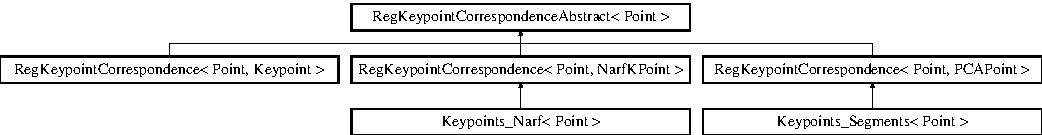
\includegraphics[height=1.818182cm]{classRegKeypointCorrespondenceAbstract}
\end{center}
\end{figure}
\subsection*{Public Member Functions}
\begin{DoxyCompactItemize}
\item 
\hypertarget{classRegKeypointCorrespondenceAbstract_aac75f2f64f77d397eb320943e4b41354}{
virtual boost::shared\_\-ptr$<$ pcl::PointCloud$<$ Point $>$ $>$ {\bfseries getSourcePoints} ()=0}
\label{classRegKeypointCorrespondenceAbstract_aac75f2f64f77d397eb320943e4b41354}

\item 
\hypertarget{classRegKeypointCorrespondenceAbstract_a114d13ab87a3a4c3e01d53002c972946}{
virtual boost::shared\_\-ptr$<$ pcl::PointCloud$<$ Point $>$ $>$ {\bfseries getTargetPoints} ()=0}
\label{classRegKeypointCorrespondenceAbstract_a114d13ab87a3a4c3e01d53002c972946}

\item 
\hypertarget{classRegKeypointCorrespondenceAbstract_a48225ab60edb7e9cdc8d162825495a11}{
virtual void {\bfseries getCorrespondences} (std::vector$<$ pcl::registration::Correspondence $>$ \&correspondences)=0}
\label{classRegKeypointCorrespondenceAbstract_a48225ab60edb7e9cdc8d162825495a11}

\item 
\hypertarget{classRegKeypointCorrespondenceAbstract_a6ecc6460024d84074efd762c4d41f7b1}{
virtual bool {\bfseries compute} (const pcl::PointCloud$<$ Point $>$ \&src, const pcl::PointCloud$<$ Point $>$ \&tgt)=0}
\label{classRegKeypointCorrespondenceAbstract_a6ecc6460024d84074efd762c4d41f7b1}

\end{DoxyCompactItemize}
\subsubsection*{template$<$typename Point$>$ class RegKeypointCorrespondenceAbstract$<$ Point $>$}



The documentation for this class was generated from the following file:\begin{DoxyCompactItemize}
\item 
common/include/registration/registration\_\-correspondence.h\end{DoxyCompactItemize}

\hypertarget{structSORT__S}{
\section{SORT\_\-S Struct Reference}
\label{structSORT__S}\index{SORT\_\-S@{SORT\_\-S}}
}
\subsection*{Public Member Functions}
\begin{DoxyCompactItemize}
\item 
\hypertarget{structSORT__S_a8347d01556e36ec1eba673aa5be5f92e}{
bool {\bfseries operator()} (const \hyperlink{structSORT__S}{SORT\_\-S} \&i, const \hyperlink{structSORT__S}{SORT\_\-S} \&j) const }
\label{structSORT__S_a8347d01556e36ec1eba673aa5be5f92e}

\end{DoxyCompactItemize}
\subsection*{Public Attributes}
\begin{DoxyCompactItemize}
\item 
\hypertarget{structSORT__S_ae7f94164d10c83193571f39091fca282}{
float {\bfseries dis}}
\label{structSORT__S_ae7f94164d10c83193571f39091fca282}

\item 
\hypertarget{structSORT__S_a85f1c6e0ef6b14c057f104fcb48f2fa9}{
int {\bfseries ind}}
\label{structSORT__S_a85f1c6e0ef6b14c057f104fcb48f2fa9}

\end{DoxyCompactItemize}


The documentation for this struct was generated from the following file:\begin{DoxyCompactItemize}
\item 
common/include/registration/impl/registration\_\-info.hpp\end{DoxyCompactItemize}

\printindex
\end{document}
